\part{设计与分析}

\section{复数电平映射}

\subsection{场景一:BMPSK}

对于场景一的信道,由于每次通信过程中$\phi$保持不变,如果我们能将信道的$\phi$估计出来,那么就能充分利用整个复平面进行电平映射。我们设计了一种引入直流偏置的相移键控映射方式,同时完成相位估计和电平映射的任务,称之为BMPSK(Biased MPSK)。

\subsubsection{映射}

\paragraph{信道分析}
\indent

我们先对场景一的信道特性进行初步分析:
\begin{equation*}
    y=x\,e^{j\phi}+n
\end{equation*}

其中$\phi$在单次通信过程中保持不变,$n$的实虚部均服从$N(0,\sigma^2)$。我们考虑采用2bit/符号的 MPSK映射方式对信道进行分析。从图1可以看出,该信道具有如下两条特性:

\begin{enumerate}
    \item 相对相位保留:发端任意相邻电平之间的夹角为90$^{\circ}$,而在收端任意相邻电平块之间的夹角也约为90$^{\circ}$,这是因为所有电平都旋转了相同的角度$\phi$;
    \item 绝对相位丢失:由于信道引入的相位旋转是随机的,故在收端我们无法判断哪一块电平对应的是00码,这本质上是由MPSK映射的旋转对称性导致的。
\end{enumerate}

\begin{figure}[h]
    \centering
    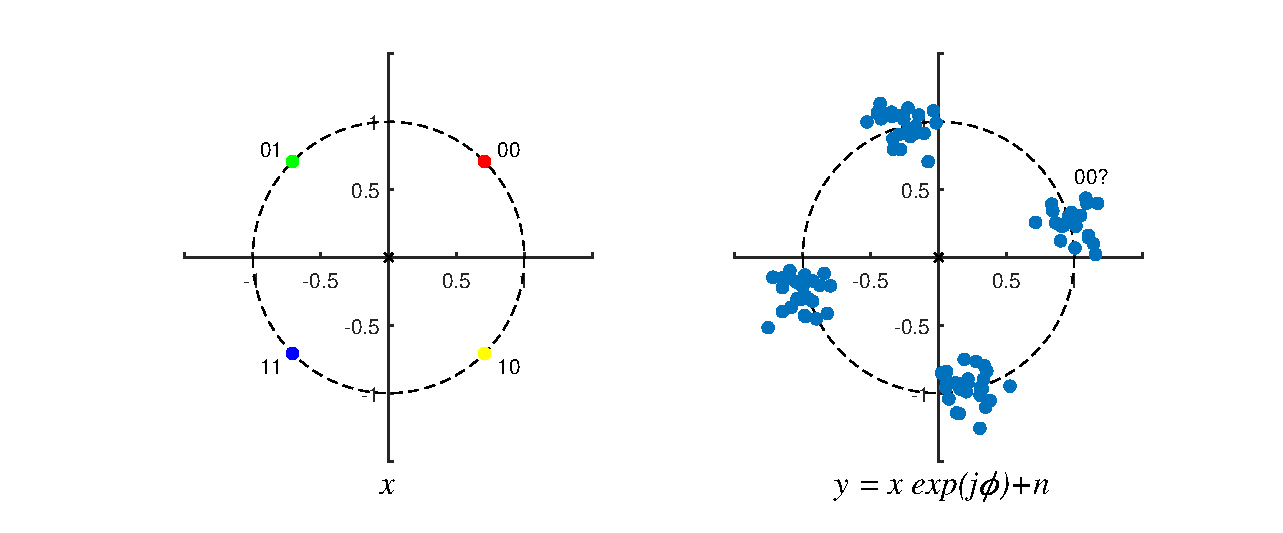
\includegraphics[width=\textwidth]{pic/1-1-1.eps}
    \caption{2bit/符号的MPSK映射收发端星座图}
\end{figure}

\paragraph{电平设计}
\indent

基于上述分析,我们认为针对场景一设计映射方式的关键在于如何估计$\phi$,如果能将信道的 $\phi$值估计出来,我们就能充分利用整个复平面进行电平映射,提高收端判决的准确度。注意到绝对相位信息丢失的根本原因是MPSK映射方式的旋转对称性,因此我们通过引入一个直流偏置来破坏其旋转对称性,从而使我们可以在收端设计方法把$\phi$估计出来。采用2bit/符号的BMPSK映射方式所得的收发端星座图如图2所示。

\begin{figure}[h]
    \centering
    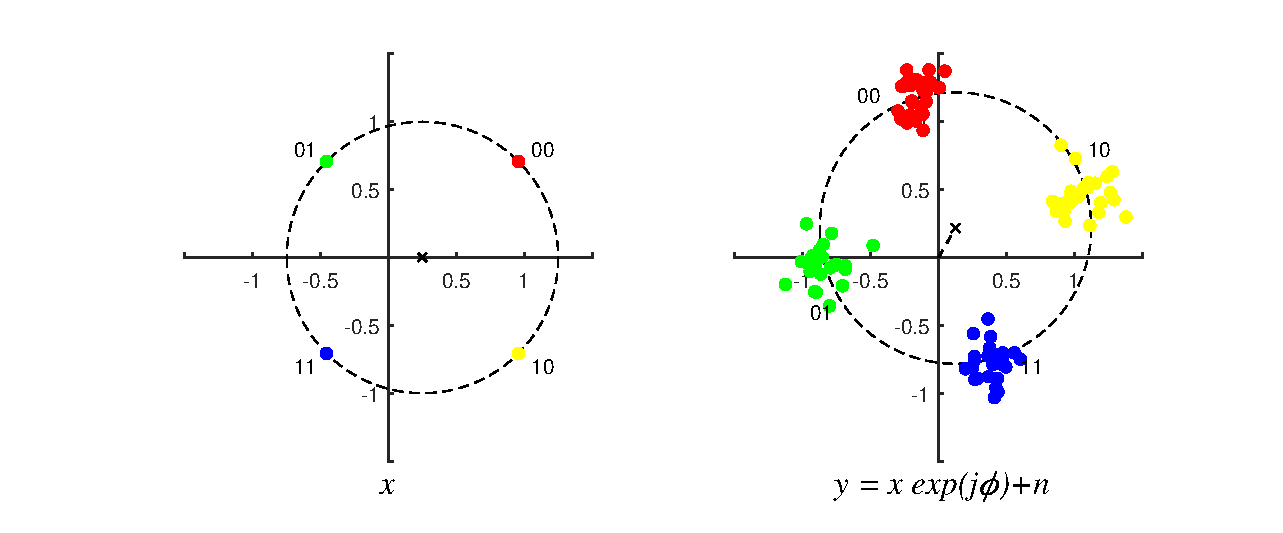
\includegraphics[width=\textwidth]{pic/1-1-2.eps}
    \caption{2bit/符号的BMPSK映射收发端星座图}
\end{figure}

从星座图上看,BMPSK实际上就是将MPSK映射所得到的电平整体向实数轴正方向移动了一段距离,我们用一个参数bias\_ratio来刻画电平的偏移程度。设MPSK映射电平的幅度为$A$,则 BMPSK电平向右移动的距离为$A\cdot bias\_ratio$。如果我们用$x_{MPSK}$表示MPSK映射方式所得到的电平,则BMPSK的映射电平$x_{BMPSK}$可以表示为:
$$x_{BMPSK}=x_{MPSK}+A\cdot bias\_ratio$$

具体而言,1bit/符号,2bit/符号,3bit/符号的BMPSK电平映射如下表所示。

\begin{table}[h]
    \centering
    \small
    \subtable[1bit/符号]{
        \begin{tabular}{c|c}
            \hline
                比特 & 映射电平 \\
            \hline
                0 & $A(e^{i\frac{\pi}{2}}+bias\_ratio)$ \\
                1 & $A(e^{i\frac{3\pi}{2}}+bias\_ratio)$ \\
            \hline
        \end{tabular}
    }
    \subtable[2bit/符号]{
        \begin{tabular}{c|c}
            \hline
                比特 & 映射电平 \\
            \hline
                00 & $A(e^{i\frac{\pi}{4}}+bias\_ratio)$ \\
                01 & $A(e^{i\frac{3\pi}{4}}+bias\_ratio)$ \\
                11 & $A(e^{i\frac{5\pi}{4}}+bias\_ratio)$ \\
                10 & $A(e^{i\frac{7\pi}{4}}+bias\_ratio)$ \\
            \hline
        \end{tabular}
    }
    \subtable[3bit/符号]{
    \begin{tabular}{c|c}
            \hline
                比特 & 映射电平 \\
            \hline
                000 & $A(e^{i\frac{\pi}{8}}+bias\_ratio)$ \\
                001 & $A(e^{i\frac{3\pi}{8}}+bias\_ratio)$ \\
                011 & $A(e^{i\frac{5\pi}{8}}+bias\_ratio)$ \\
                010 & $A(e^{i\frac{7\pi}{8}}+bias\_ratio)$ \\
                110 & $A(e^{i\frac{9\pi}{8}}+bias\_ratio)$ \\
                111 & $A(e^{i\frac{11\pi}{8}}+bias\_ratio)$ \\
                101 & $A(e^{i\frac{13\pi}{8}}+bias\_ratio)$ \\
                100 & $A(e^{i\frac{15\pi}{8}}+bias\_ratio)$ \\
            \hline
        \end{tabular}
    }
    \caption{BMPSK电平映射表}
\end{table}

\subsubsection{判决}

\paragraph{相位估计}
\indent

进行判决的第一步是对$\phi$进行估计,我们的估计方法基于如下两个观察:

\begin{enumerate}
    \item 发端映射电平的期望是引入偏置后映射电平所在圆的圆心,这个圆心为$A\cdot bias\_ratio$。其推导过程为:
    $$E(x_{BMPSK})=E(x_{MPSK}+A\cdot bias\_ratio)
    =A\cdot bias\_ratio$$
    \item 收端电平的期望也是一个圆的圆心,这个圆是发端圆绕原点旋转$\phi$所得到的圆,故其圆心为$A\cdot bias\_ratio\cdot e^{j\phi}$。其推导过程为:
    $$E(y)=E(x_{BMPSK}e^{j\phi}+n)=A\cdot bias\_ratio\cdot e^{j\phi}$$
\end{enumerate}

\begin{figure}[h]
    \centering
    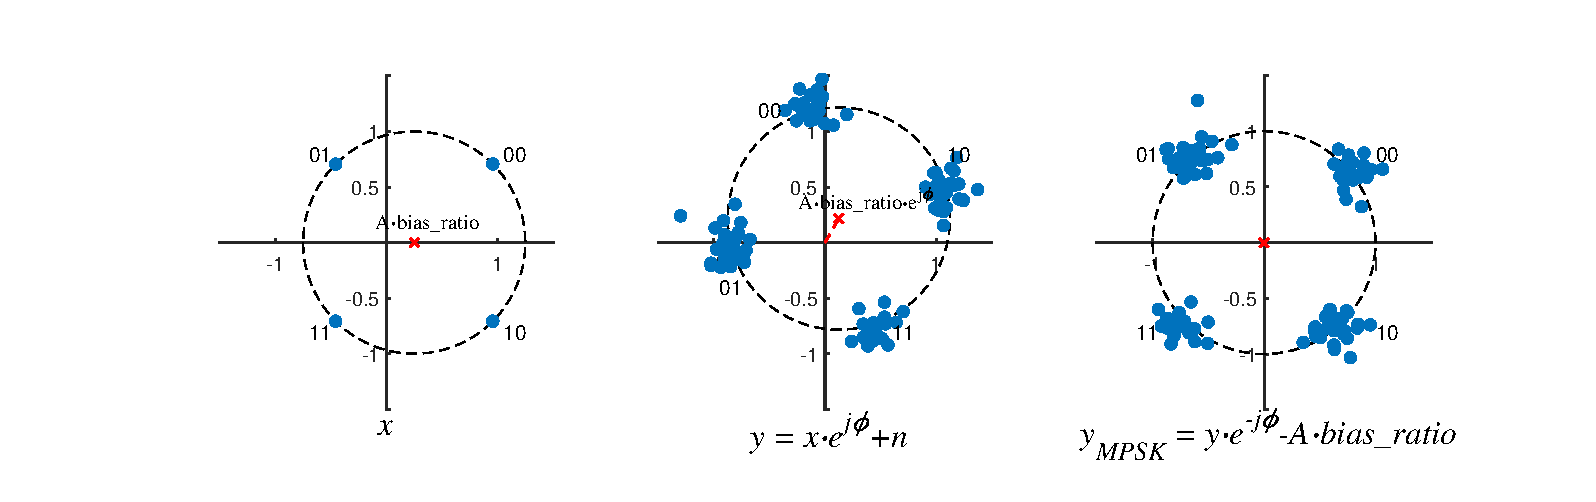
\includegraphics[width=\textwidth]{pic/1-1-3.eps}
    \caption{相位估计与恢复过程}
\end{figure}

上式建立起了$E(y)$与$\phi$之间的关系,由此我们可以反解出:
$$\phi=angle(E(y))$$

注意到在实际通信中我们不可能知道$E(y)$,因此我们通过求$y$的均值来对其进行近似,从而估计出$\phi$:
$$\phi=angle(E(y))\approx angle(\frac{1}{n}\sum_{i=1}^ny_i)$$

在估计出$\phi$后,我们就可以对$y$进行一定的预处理:先将$y$反向旋转角度$\phi$,再将其向实数轴负方向平移$A\cdot bias\_ratio$。即:
$$\tilde{y}=y\cdot e^{-j\phi}-A\cdot bias\_ratio$$

如果我们的$\phi$估计得足够准确,那么预处理后的$\tilde{y}$就等价于标准的MPSK映射电平经过一个高斯信道后的收端电平,从而便于我们进行之后的电平判决。

\paragraph{判据推导}
\indent

在判据的推导中,我们近似地认为经过预处理后的$\tilde{y}$等价于标准的MPSK映射电平经过一个高斯信道后的收端电平。在下面的的推导中,我们用$\tilde{x}$表示MPSK的映射电平,则基于最大后验概率的判据为:
\begin{equation*}
\begin{aligned}
    P(\tilde{x}|\tilde{y})
    &=\frac{P(\tilde{x})P(\tilde{y}|\tilde{x})}{P(\tilde{y})}
    =\frac{P(\tilde{x})}{P(\tilde{y})}P(n=\tilde{y}-\tilde{x})\\
    &=\frac{P(\tilde{x})}{P(\tilde{y})}
    P(real(n)=real(\tilde{y}-\tilde{x}))
    P(imag(n)=imag(\tilde{y}-\tilde{x}))\\
    &=\frac{P(\tilde{x})}{P(\tilde{y})}
    f(real(n)=real(\tilde{y}-\tilde{x}))
    f(imag(n)=imag(\tilde{y}-\tilde{x}))\\
    &=\frac{P(\tilde{x})}{P(\tilde{y})}
    \frac{1}{\sqrt{2\pi\sigma^2}}
    e^{-\frac{(real(\tilde{y}-\tilde{x}))^2}{2\sigma^2}}
    \frac{1}{\sqrt{2\pi\sigma^2}}
    e^{-\frac{(imag(\tilde{y}-\tilde{x}))^2}{2\sigma^2}}\\
    &=\frac{P(\tilde{x})}{P(\tilde{y})}
    \frac{1}{2\pi\sigma^2}
    e^{-\frac{||\tilde{y}-\tilde{x}||^2}{2\sigma^2}}
\end{aligned}
\end{equation*}

注意到对于任意的$\tilde{x}$和固定的$\tilde{y}$,我们有$\frac{P(\tilde{x})}{P(\tilde{y})}$为定值,故有:
$$P(\tilde{x}_i|\tilde{y})\leq P(\tilde{x}_j|\tilde{y})\Leftrightarrow ||\tilde{y}-\tilde{x}_i||\geq||\tilde{y}-\tilde{x}_j||$$

即基于最大后验概率的判决等价于基于欧氏距离的判决。而对于MPSK的映射方式,基于欧氏距离的判决等价于基于$\tilde{y}$的辐角的判决:以2bit/符号的MPSK映射为例,其任意相邻电平的中垂线可以用极坐标表示为$\theta_k=k\pi/2,\,k=0,1,2,3$,这些射线将复平面平均划分为4个部分,因此在实现的过程中,我们可以方便地通过$\tilde{y}$的辐角对其发射电平进行判决。综上所述,电平判据的结论为:

\begin{center}
    基于最大后验概率的判决 $\Leftrightarrow$ 基于欧氏距离的判决 $\Leftrightarrow$ 基于电平辐角的判决 
\end{center}

\begin{figure}[h]
    \centering
    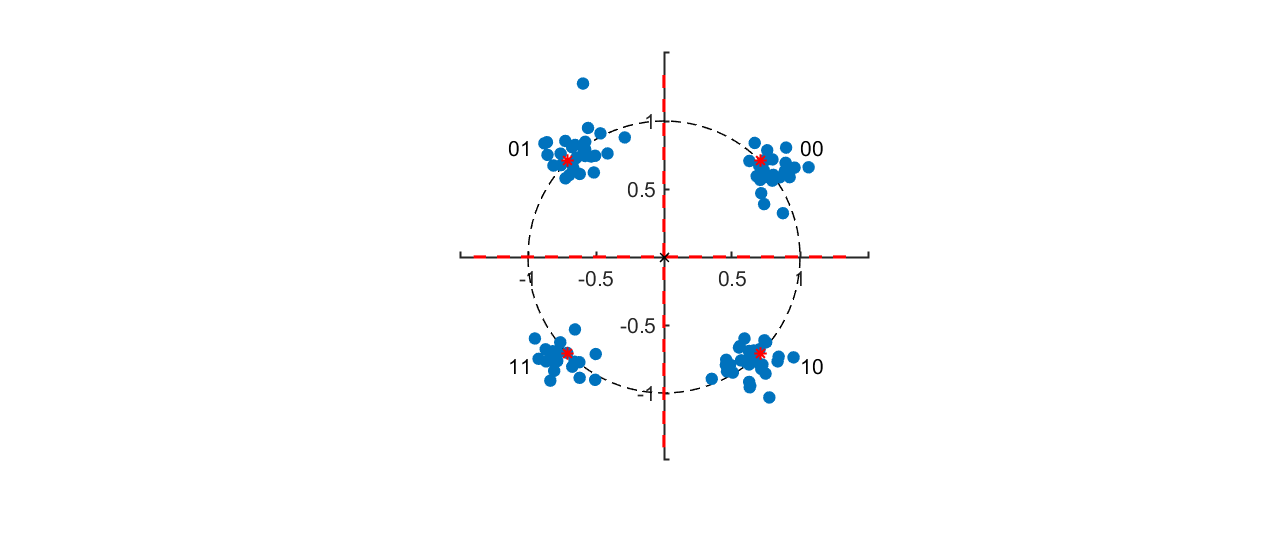
\includegraphics[width=\textwidth]{pic/1-1-4.eps}
    \caption{2bit/符号的BMPSK电平判决}
\end{figure}


\paragraph{仿真结果}
\indent

在仿真中,我们生成了长度为100,000bit的随机序列,设置偏置系数bias\_ratio=1/4,分别采用1bit/符号,2bit/符号,和3bit/符号的BMPSK映射方式,得到了如下的BER-SNR曲线,其中左边的图为线性坐标,右边的图为对数坐标:

\begin{figure}[ht]
    \centering
    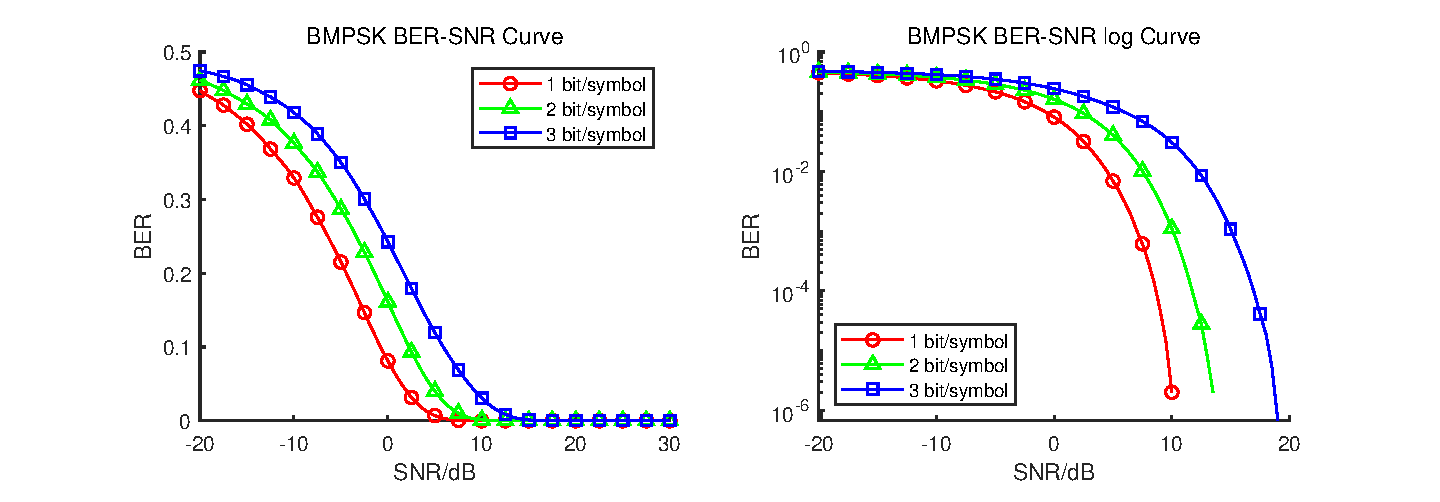
\includegraphics[width=\textwidth]{pic/1-1-5.eps}
    \caption{1,2,3 bit/符号映射时BMPSK的BER-SNR曲线}
\end{figure}

从左边的线性坐标的图中可以看出:在相同信噪比的条件下,1bit/符号映射的误码率小于 2bit/符号映射的误码率小于3bit/符号映射的误码率。这样的结果是符合我们的预期的,因为每符号对应的比特数越多,意味着我们在相同半径的圆周上放置的电平越多,也就意味着在相同噪声下我们区分不同电平的能力下降,故误码率上升。

从右边的对数坐标的图中可以看出:1bit/符号映射的误码率在信噪比约为10dB时降为$10^{-6}$,2bit/符号的相应信噪比大约为15dB,3bit/符号的相应信噪比大约为20dB。

\subsubsection{折衷}

在BMPSK的设计中,我们使用了bias\_ratio这个参数来刻画信号电平的偏移程度,该参数的取值直接影响了BMPSK映射的性能。从相位估计和信号功率两个角度,我们对参数bias\_ratio提出了不同的要求,因此在实际使用中,我们需要对bias\_ratio的取值进行折衷,从而获得最优的映射与判决性能。

\paragraph{精度分析}
\indent

从相位估计的角度考虑,bias\_ratio越大,相位估计得越准。在相位估计部分的推导中,我们从期望的角度考虑,完全忽略了高斯白噪声$n$对于相位估计的影响。而在实际情况中,我们对信道相位$\phi$的估计应修改为:
\begin{equation*}
\begin{aligned}
    \tilde{\phi}&=angle(mean(y))
    \approx angle(A\cdot bias\_ratio\cdot e^{j\phi}+mean(n))\\
    &=angle(A\cdot e^{j\phi}+\frac{mean(n)}{bias\_ratio})
\end{aligned}
\end{equation*}

注意到在传输有限个电平时,$mean(n)$的值不等于0,因此在实际的传输过程中,高斯白噪声$n$会对相位$\phi$的估计带来一定的误差。而观察上式可知,在$n$确定的情况下,bias\_ratio的值越大,误差项$\varepsilon=\frac{mean(n)}{bias\_ratio}$对相位估计带来的误差就越小。这在直观理解上也是非常合理的,因为bias\_ratio越大,意味着偏置后圆心的模长越大,也就意味着其抗噪声的能力越强,因此相位就估计越准。

在仿真中,我们分别设置bias\_ratio的值为1/16,1/4,和1,并生成了长度为100,000bit的随机序列,采用2bit/符号的BMPSK映射方式,作出了信道相位的估计值与真值的误差$\Delta\phi=|\phi-\tilde{\phi}|$随信噪比变化的曲线。该仿真结果也验证了我们得到的bias\_ratio越大,相位估计越准的分析结果。

\begin{figure}[h]
    \centering
    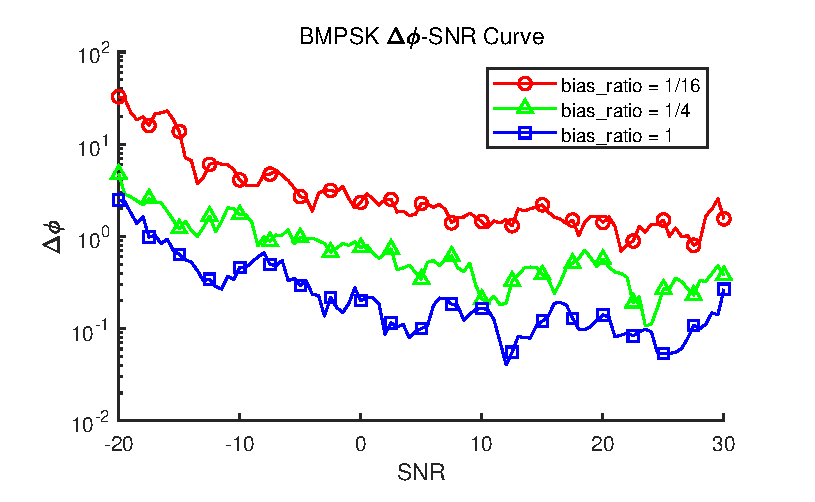
\includegraphics[width=0.6\textwidth]{pic/1-1-6.eps}
    \caption{BMPSK $\Delta\phi$-SNR曲线}
\end{figure}

\paragraph{功率分析}
\indent

从信号功率的角度考虑,bias\_ratio越小,信号功率越小。直观理解的理解是,bias\_ratio越大,意味着需要的直流偏置功率越大,而引入的直流偏置并没有给我们带来更多的信息,因此从理论上讲误码率并不会发生任何变化。我们也可以从理论上进行严格的推导,考虑电平个数为M的BMPSK映射方式,其信号的功率为:
\begin{equation*}
\begin{aligned}
    P_S&=\frac{1}{M}\sum_{k=1}^M||S_k||^2
    =\frac{1}{M}\sum_{k=1}^M||A\cdot(e^{\theta_k}
    +bias\_ratio)||^2\\
    &=\frac{A^2}{M}\sum_{k=1}^M((cos\theta_k+bias\_ratio)^2
    +sin^2\theta_k)\\
    &=\frac{A^2}{M}(\sum_{k=1}^M(1+bias\_ratio^2)
    +2\cdot bias\_ratio\sum_{k=1}^M cos\theta_k)\\
    &=A^2(1+bias\_ratio^2)
\end{aligned}
\end{equation*}

由上述推导可知,信号功率$P_S$正比于1+bias\_ratio$^2$。由于我们考虑信噪比时通常取对数,而在bias\_ratio$\in[0,1]$时,$log(P_S)$近似正比于bias\_ratio,如下图所示:

\begin{figure}[h]
    \centering
    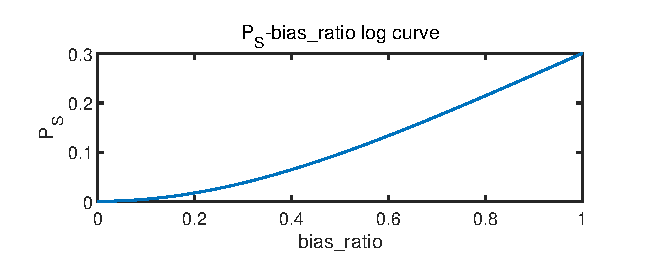
\includegraphics[width=0.5\textwidth]{pic/1-1-7.eps}
    \caption{$P_S-bias\_ratio$关系曲线}
\end{figure}

\paragraph{仿真结果}
\indent

从相位估计和信号功率两个不同的角度,我们对参数bias\_ratio提出了不同的要求,因此在实际使用中我们需要对bias\_ratio的取值进行折衷,从而获得最优的映射与判决性能。在仿真中,我们分别设置bias\_ratio为1/16,1/4,和1,并生成了长度为5,000bit的随机序列,采用2bit/符号的BMPSK映射方式,得到了如下的BER-SNR曲线,其中左边的图为线性坐标,右边的图为对数坐标:

\begin{figure}[h]
    \centering
    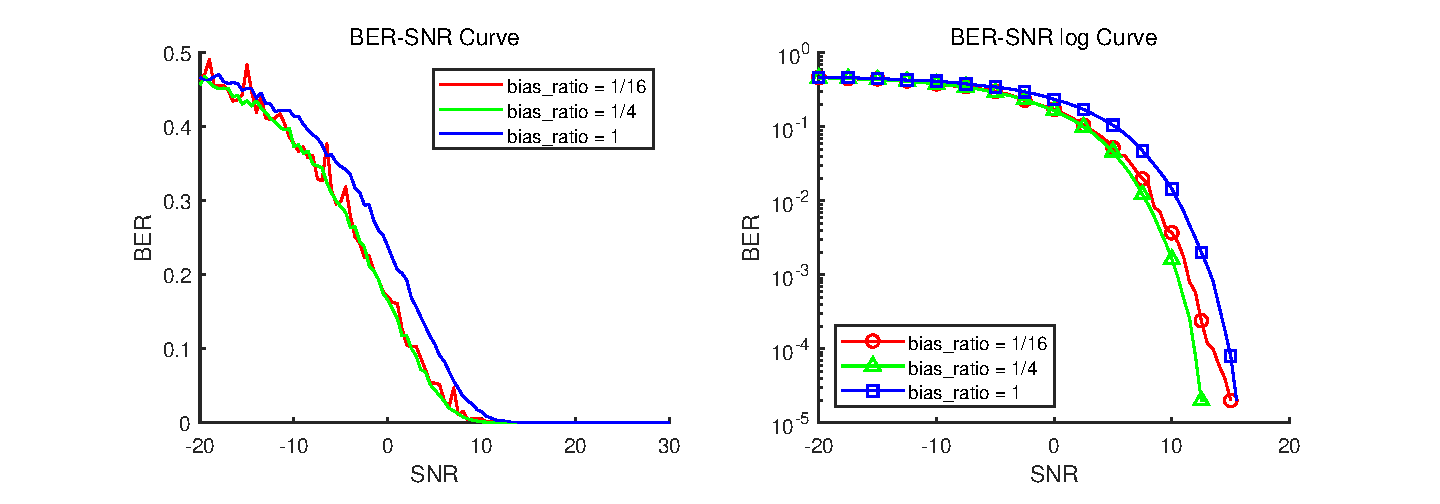
\includegraphics[width=\textwidth]{pic/1-1-8.eps}
    \caption{bias\_ratio=1/16,1/4,1时BMPSK的BER-SNR曲线}
\end{figure}

从左边的线性坐标的图中可以看出:红线代表的bias\_ratio=1/16时的BER-SNR曲线有非常明显的抖动,从我们上述对于$\phi$的精度分析可知,这是由于bias\_ratio的取值太小,导致我们对$\phi$的估计的方差较大,鲁棒性不够强;而在误码率相同的情况下,蓝线代表的bias\_ratio=1时功率始终大于绿线代表的bias\_ratio=1/4时的功率,这与我们上述对于信号功率的分析结果是一致的。

从右边的对数坐标的图中可以看出:绿线代表的bias\_ratio=1/4时的误码率是三种情况中的最小值,因此综合分析,我们认为折衷选取的1/4是一个比较合理的参数值。在经过多次仿真后,我们最后确定当bias\_ratio的取值在1/8到1/4之间时,BMPSK的映射方式具有较好的性能。

\subsection{场景一:PHIMAP}

由于BMPSK算法是将$\phi$的估计和电平映射耦合在一起的算法。因此,我们想要提出一个方法,能够独立的估计出$\phi$,之后我们可以使用现有的任何一种电平映射方法,如PSK等。

我们估计$\phi$的算法基于这样的一种直观的想法。我们的发送和接收双方,在每次通信前约定,发送一个固定的符号序列$X=\{X_1,X_2,\cdots,X_n\}$。同时,接收方观测到了一个符号序列 $Y=\{Y_1,Y_2,\cdots,Y_n\}$。之后,我们计算出给定X和观测到Y的$\phi$的后验概率$P(\phi|X,Y)$,就能求出最大化后验概率的估算值及其期望的误差。

经过推导,我们有估计值$\phi^*$
\begin{equation*}
    \phi^{*}=\phi_K
\end{equation*}

其中有:
\begin{equation*}
\begin{aligned}
    & K_1=\frac{\sum\limits_{i=1}^n |X_i||Y_i|cos\phi_i}{\sigma^2}&\,\,\,\,
    K_2=\frac{\sum\limits_{i=1}^n |X_i||Y_i|sin\phi_i}{\sigma^2}\\
    & cos\phi_K=\frac{K_1}{\sqrt{K_1^2+K_2^2}}&\,\,\,\,
    sin\phi_K=\frac{K_2}{\sqrt{K_1^2+K_2^2}}
\end{aligned}
\end{equation*}

同时,我们估计的偏差的期望值$E(|\epsilon||X,Y)$为
\begin{equation*}
    E(|\epsilon||X,Y)=\frac{\int_{-\pi}^\pi |\epsilon| exp(K_3cos\epsilon+K_4sin\epsilon) \mathrm{d}\epsilon}{\int_{-\pi}^\pi exp(K_3cos\epsilon+K_4sin\epsilon) \mathrm{d}\epsilon}\
\end{equation*}

其中有
\begin{equation*}
\begin{aligned}
    K_3&=\frac{\sum\limits_{i=1}^n |X_i||Y_i|cos(\phi_i-\phi^*)}{\sigma^2}\,\,\,\,
    K_4&=\frac{\sum\limits_{i=1}^n |X_i||Y_i|sin(\phi_i-\phi^*)}{\sigma^2}
\end{aligned}
\end{equation*}

PHIMAP算法和BMPSK在给定所有条件相同的时候,有一样的性能。并且对$\phi$的估计都十分准确,不存在由于$\phi$的估计而引入的误差。如果允许PHIMAP算法多发送50个符号,那么在低信噪比下比BMPSK算法性能略好一些,这主要是因为两个算法符号能量不同。BMPSK有一个直流偏置,能量略大一些,因此在相同信噪比和相同发射功率下,他的能量更高。此外,PHIMAP 和BMPSK应该使用哪个算法,应该由我们的需求和我们的限制决定,各有优劣。

\subsection{场景二:ASK}

对于场景二的信道,每次通信过程中$\phi$均独立变化,此时调制在电平相位上的信息将会全部损失。故在这种情况下,我们只能利用复数电平的幅度信息。考虑采用不归零的幅度键控(ASK) 的调制方式。1bit/符号时使用2ASK,2bit/符号时使用4ASK,3bit/符号时使用8ASK,在映射时采用格雷码编码,选择均匀分布。具体映射如下表所示:

\begin{table}[h]
    \centering
    \small
    \subtable[2ASK]{
        \begin{tabular}{c|c}
            \hline
                比特 & 映射电平 \\
            \hline
                0 & $0$ \\
                1 & $A$ \\
            \hline
        \end{tabular}
    }
    \subtable[4ASK]{
        \begin{tabular}{c|c}
            \hline
                比特 & 映射电平 \\
            \hline
                00 & $0$ \\
                01 & $\frac{A}{3}$ \\
                11 & $\frac{2A}{3}$ \\
                10 & $A$ \\
            \hline
        \end{tabular}
    }
    \subtable[8ASK]{
        \begin{tabular}{c|c}
            \hline
                比特 & 映射电平 \\
            \hline
                000 & $0$ \\
                001 & $\frac{A}{7}$ \\
                011 & $\frac{2A}{7}$ \\
                010 & $\frac{3A}{7}$ \\
                110 & $\frac{4A}{7}$ \\
                111 & $\frac{5A}{7}$ \\
                101 & $\frac{6A}{7}$ \\
                100 & $A$ \\
            \hline
        \end{tabular}
    }
    \caption{2ASK、4ASK、8ASK映射关系表}
\end{table}
其中A为符号电平的幅值。

再考虑从经过信道的电平符号解调出比特,判决时应采用最大后验概率准则(MAP),在各电平符号等概时等价于最大似然准则(ML)。但最大似然准则并不能等价于最小欧氏距离准则。下图为2bit/符号的ASK在收发两端以及判决时的星座图:
\begin{figure}[h]
    \centering
    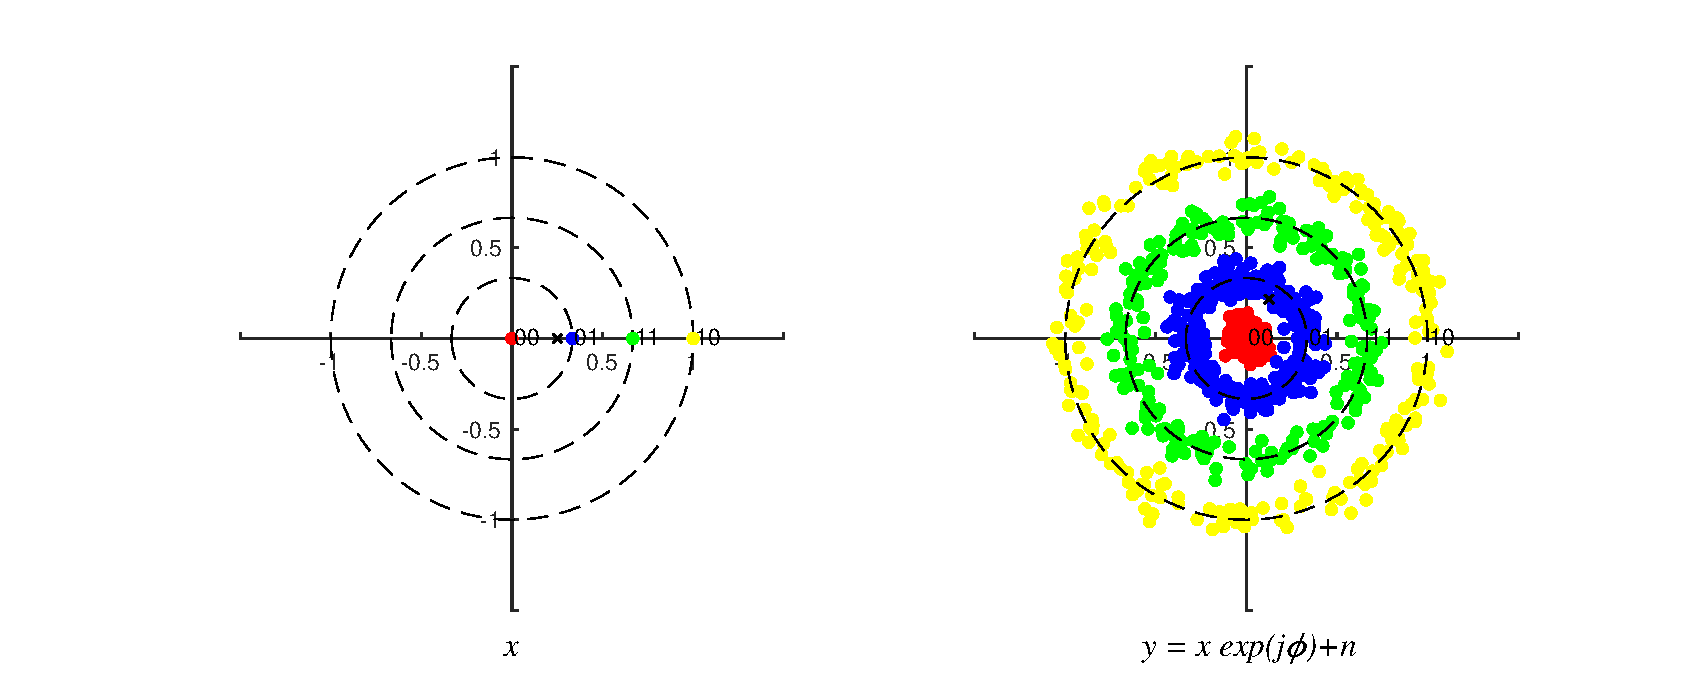
\includegraphics[width=0.8\textwidth]{pic/ASK_con.eps}
    \caption{2bit/符号 ASK星座图}
\end{figure}

经推导得,判决可用以下形式表述
\begin{equation*}
    a^*=\mathop{\arg\max}_{a\in\{A\}}f(a,r)=\mathop{\arg\max}_{a\in\{A\}}I_0(\frac{ar}{\sigma^2})e^{-\frac{a^2}{2\sigma^2}}
\end{equation*}

可以利用二分法和对数压缩的方法逼近得到各个判决门限。

\begin{figure}[h]
    \centering
    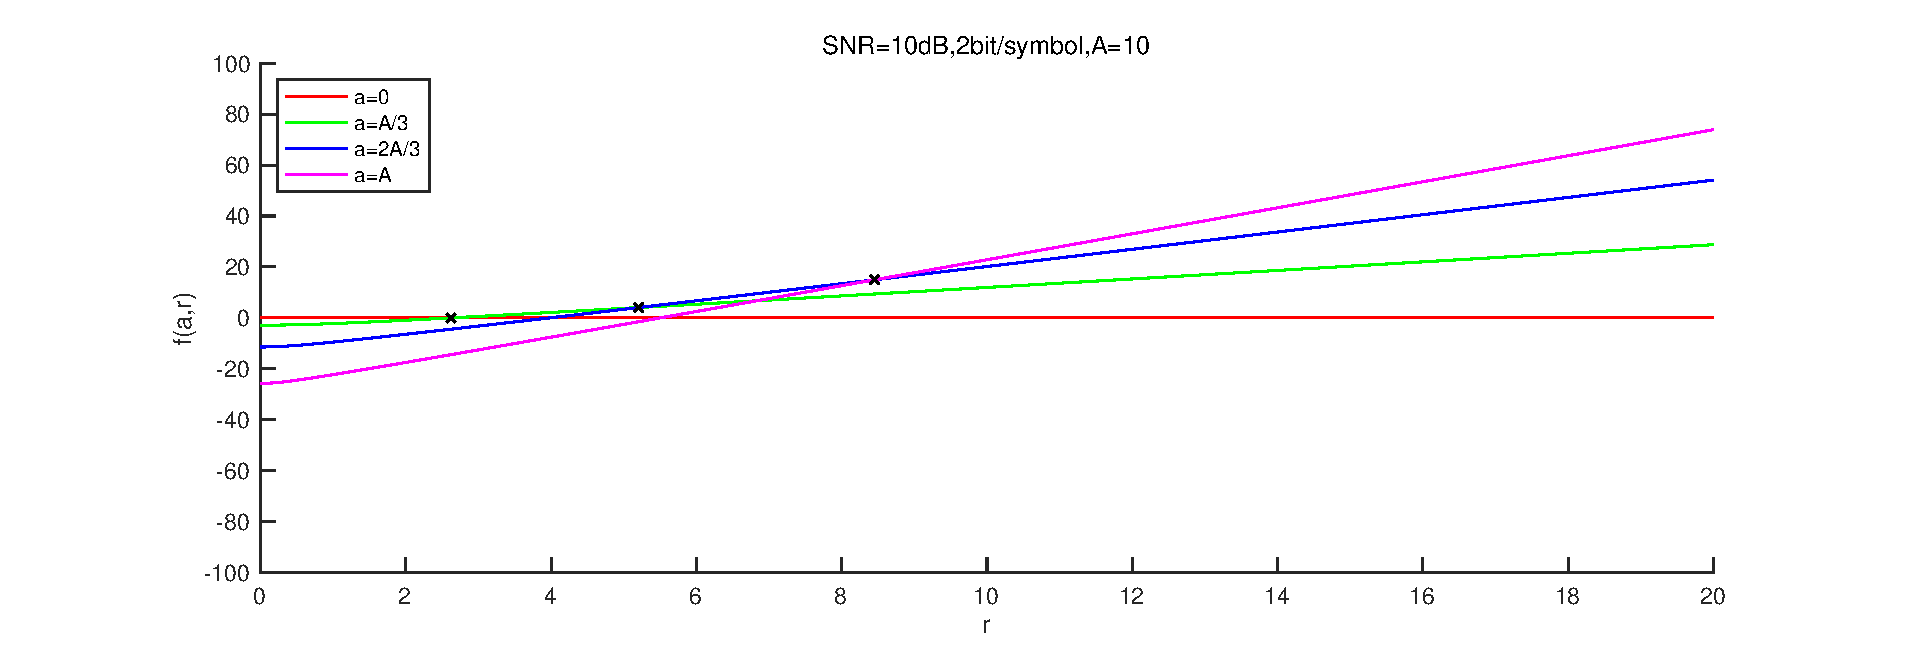
\includegraphics[width=0.8\textwidth]{pic/threshold.eps}
    \caption{二分法逼近得到判决门限}
\end{figure}

通过数值仿真可以比较基于最大似然准则和基于最小欧氏距离准则的性能,具体结果如下图所示:

\begin{figure}[h]
    \centering
    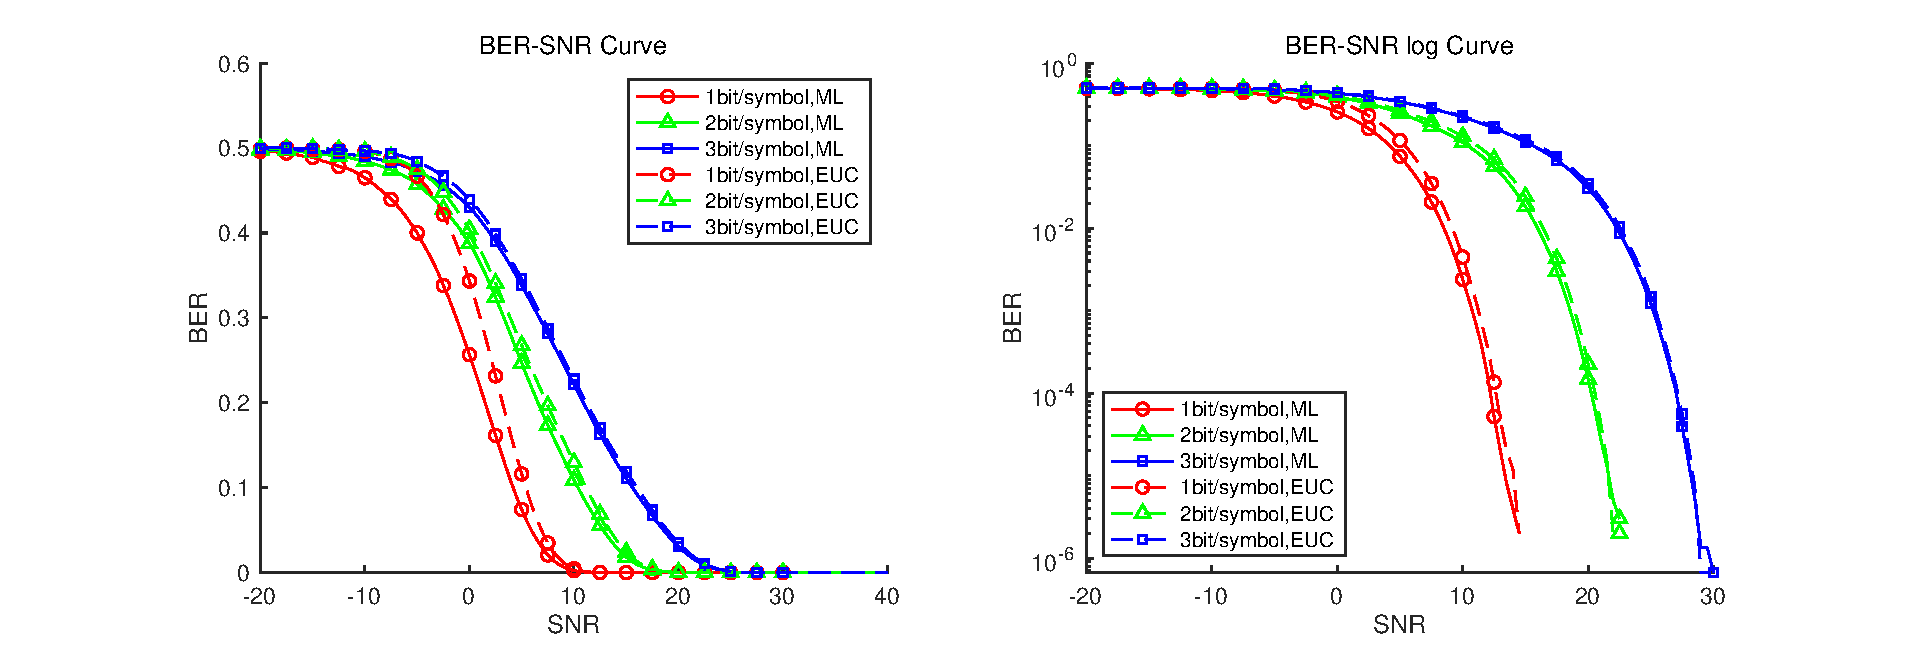
\includegraphics[width=0.8\textwidth]{pic/ASK_SNR_BER.eps}
    \caption{基于ML和EUC准则下ASK的SNR-BER曲线}
\end{figure}

前者的性能在各种bit/符号的情况下都优于后者,在1bit/符号时尤为明显,这主要是因为此时各复数电平间距较大,因此最大似然判据相较于最小欧氏距离的改善更为显著。

\section{卷积码编译码}

卷积码是一种有记忆的信道编码,其编译码原理在理论课上已有详细介绍,下面我们仅讨论其算法思路与实现过程。

\subsection{编码模块}

卷积码编码的思路较为简单直观,我们在这里仅讨论其实现过程。

\subsubsection{收尾情况}

收尾情况下卷积码编码模块的实现过程可以分为以下3个步骤:

\begin{enumerate}
    \item 设置多项式系数:我们用一个系数矩阵coeff储存卷积码编码的多项式系数,注意到1/2效率 (15,17)编码和1/3效率(13,15,17)多项式可以统一地使用一个系数矩阵表示:
    \begin{equation*}
    coeff=\left[
        \begin{matrix}
            1 & 0 & 1 & 1\\
            1 & 1 & 0 & 1\\
            1 & 1 & 1 & 1
        \end{matrix}
    \right]
    \end{equation*}
    该矩阵的2,3行用于1/2效率的(15,17)编码,1,2,3行用于1/3效率的(13,15,17)编码。事实上,我们可以容易地将该固定多项式系数的卷积码编码模块扩展为任意多项式系数的编码模块,只需要将系数矩阵coeff作为一个可调的输入参数即可实现;
    \item 逐参数卷积:对于1/n效率的编码,我们用一个n$\times$(len+4)的矩阵code来储存卷积后得到的码字,其中len为待编码比特串data的长度。我们用code矩阵的第i行用于储存data经第i个多项式系数卷积后得到的码字,因此可以逐参数地调用conv()函数进行卷积编码。注意到收尾的要求和conv()函数本身的计算范围,我们只需要在data的末尾添上一个0;
    \item 重构卷积码矩阵:因为卷积码编码模块应按照输入顺序依次输出各比特卷积编码后得到的 n bit卷积码,因此我们需要将原大小为n$\times$(len+4)的矩阵code重构为1$\times$(len+4)n的比特串,我们可以通过调用reshape()函数来实现这一过程。
\end{enumerate}

\subsubsection{不收尾情况}

不收尾的情况不需要在待卷积比特串data的末尾添上4个0,这等价于去掉卷积码code的最后 4n位码字。在实现中,我们先统一地按照收尾情况对data进行处理,若为不收尾的情况,只需要将输出卷积码code末尾的4n位码字去掉即可。

\subsection{译码模块}

卷积码译码的算法采用了Viterbi算法。Viterbi算法本质上是一个动态规划的算法,我们在实现中分别使用了一个向量和一个矩阵来储存各状态的累加距离和幸存路径矩阵。卷积码译码又可以分为硬判决译码和软判决译码,其中硬判决译码的输入为经历了电平判决后的码字,故采用汉明距离度量;而软判决译码的输入为未经电平判决前的复数电平,故采用欧氏距离度量。

\subsubsection{硬判决译码}

硬判决译码有1/2效率和1/3效率两种情况,其实现过程均可以分为以下3个步骤:

\begin{enumerate}
    \item 初始化:初始化各状态的累加汉明距离hamm\_dist。因为卷积码编码的起始状态只能为000 状态,因此我们将hamm\_dist初始化为:
    $$hamm\_dist=[
    \begin{matrix}
        0 & +\infty & +\infty & +\infty &
        +\infty & +\infty & +\infty & +\infty
    \end{matrix}
    ]$$
    \item 循环译码:在译码结束前,循环执行以下操作
    \begin{enumerate}
        \item 计算单步汉明距离:根据卷价码效率读取n bit待译码字,计算其与各单步状态转移路径对应的许用码字之间的汉明距离向量curr\_dist;
        \item 更新累加汉明距离:将各状态此前的累加汉明距离与单步汉明距离相加,选取各状态当前的最短累加汉明距离,并更新hamm\_dist向量;
        \item 记录幸存路径:将各状态当前最短累加汉明距离对应的单步源状态写入幸存路径矩阵 survive\_path。
    \end{enumerate}
    \item 回溯:先根据是否收尾确定回溯起点,若不收尾,则选择最终累加汉明距离最小的状态作为回溯起点;若收尾,则选择00状态作为回溯起点。再根据幸存路径矩阵survive\_path逐步回溯当前时刻的源状态,并输出译码结果。
\end{enumerate}

下图为硬判决单步译码过程的示意图。为了作图的方便和清晰,我们在这里仅以4状态的硬判决译码为例说明算法执行过程:

\begin{figure}[h]
    \centering
    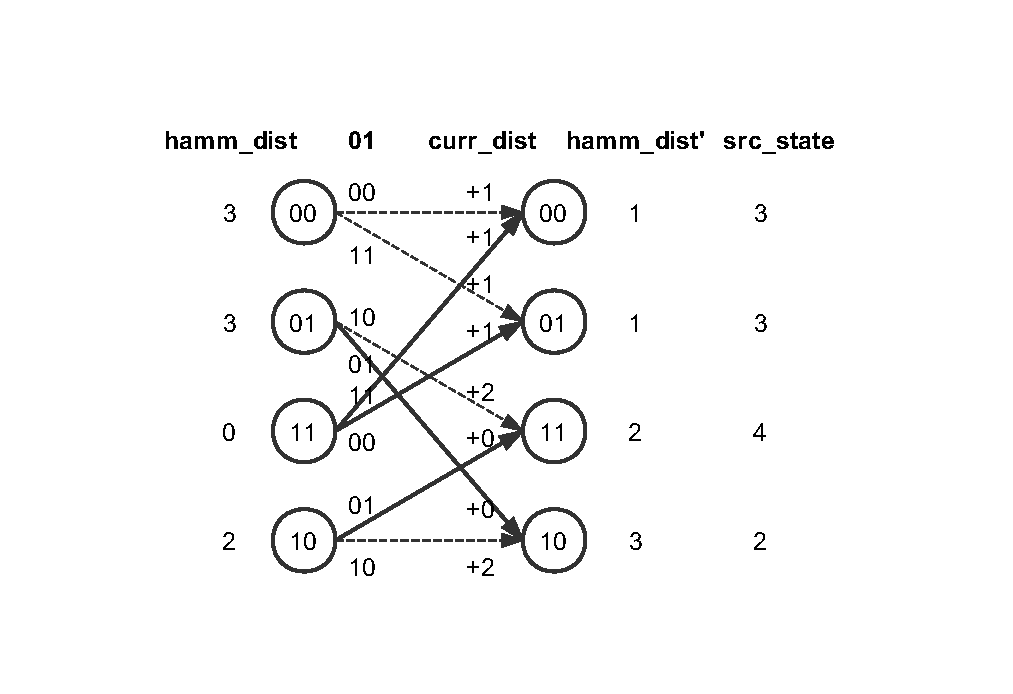
\includegraphics[width=0.6\textwidth,trim=0 40 0 40,clip]{pic/2-2-1.eps}
    \caption{硬判决单步译码过程}
\end{figure}

\subsubsection{软判决译码}

软判决算法的设计思路与硬判决并没有本质的差别,但其难点在于卷积模块与电平映射模块的组合一共存在2种卷积效率$\times$3种映射比特数=6种可能的情况,而各情况下软判决译码的处理过程是有所不同的。为了便于讨论,我们记(n,m)为1/n卷积效率,m bit/符号的模块组合情况,下面逐情况对其软判决算法进行分析。

\paragraph{(2,2)和(3,3)}
\indent

(2,2)和(3,3)的组合是最简单的情况。在这种情况下,读入1个复数电平后恰好可以译出1位码字,故此时软判决的实现过程与硬判决并没有本质的差别,我们只需要将循环译码中的距离度量方式从码字间的汉明距离变为电平间的欧氏距离。事实上,我们可以使用任何一种距离度量的方式来实现软判决译码,这也保证了我们程序的可扩展性。

该组合情况下软判决译码的实现过程可以分为以下3个步骤:

\begin{enumerate}
    \item 初始化:初始化各状态的累加欧氏距离eucd\_dist。因为卷积码编码的起始状态只能为000 状态,因此我们将eucd\_dist初始化为:
    $$eucd\_dist=[
    \begin{matrix}
        0 & +\infty & +\infty & +\infty &
        +\infty & +\infty & +\infty & +\infty
    \end{matrix}
    ]$$
    \item 循环译码:在译码结束前,循环执行以下操作
    \begin{enumerate}
        \item 计算单步欧氏距离:读取1个收端电平,计算其与各单步状态转移路径的许用码字对应的复数电平之间的欧氏距离向量curr\_dist;
        \item 更新累加欧氏距离:将各状态此前的累加欧氏距离与单步欧氏距离相加,选取各状态当前的最短累加欧氏距离,并更新eucd\_dist向量;
        \item 记录幸存路径:将各状态当前最短累加欧氏距离对应的单步源状态写入幸存路径矩阵 survive\_path。
    \end{enumerate}
    \item 回溯:先根据是否收尾确定回溯起点,若不收尾,则选择最终累加欧氏距离最小的状态作为回溯起点;若收尾,则选择00状态作为回溯起点。再根据幸存路径矩阵survive\_path逐步回溯当前时刻的源状态,并输出译码结果。
\end{enumerate}

下图为软判决单步译码过程的示意图。为了作图的方便和清晰,我们在这里仅以(2,2)情况下4状态的软判决译码为例说明算法执行过程:

\begin{figure}[h]
    \centering
    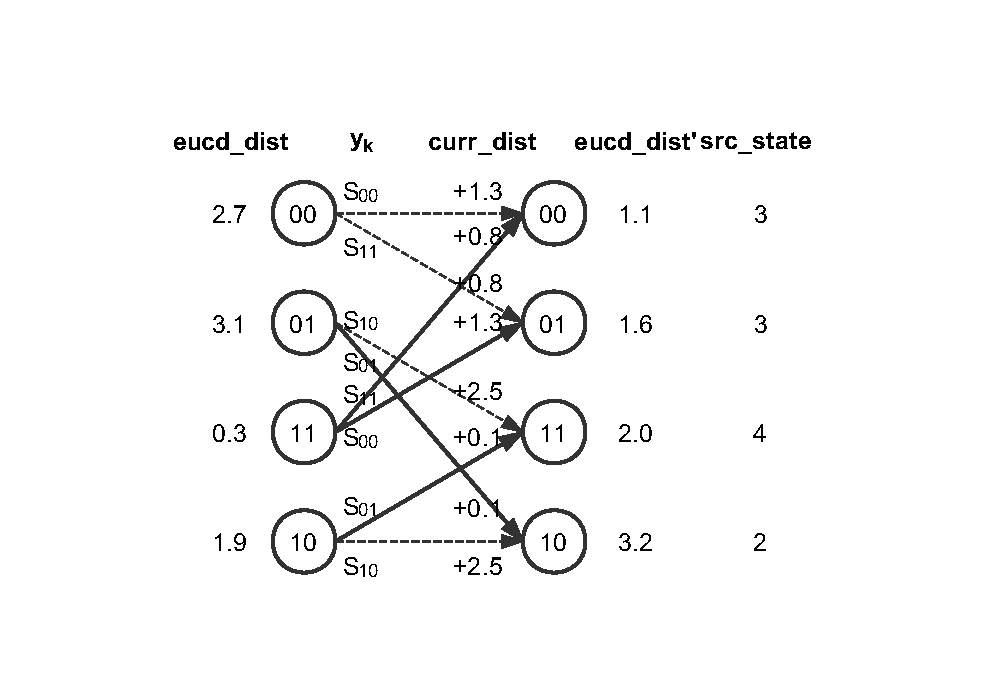
\includegraphics[width=0.6\textwidth,trim=0 40 0 40,clip]{pic/2-3-1.eps}
    \caption{(2,2)情况下软判决单步译码过程}
\end{figure}

\paragraph{(2,1)和(3,1)}
\indent

(2,1)和(3,1)的组合也是相对容易的情况。在这种情况下,读入n(n=2, 3)个复数电平后恰好可以译出1位码字,故此时软判决的实现过程只需要将循环译码中的计算单步欧氏距离的操作修改为:读取n个收端电平,计算其与各单步状态转移路径的许用码字对应的n个复数电平间的欧氏距离向量curr\_dist。

\paragraph{(2,3)和(3,2)}
\indent

(2,3)和(3,2)的组合是两种相对复杂的情况。以(3,2)的组合为例,每个复数电平对应了2位卷积码字,而需要3位卷积码字才能译出1位原码字,因此我们需要一次读入3个收端电平,这3个电平共同对应了6位卷积码字,通过这6位卷积码字我们可以译出2位原码字,下图为(3,2)情况下软判决读入3个电平译出2位码字的两步译码过程示意图。因此在(2,3)或(3,2)的组合情况下,我们需要在一次循环译码中发生了多步状态转移,这样的软判决译码实现无法用之前情况的简单推广解决。

\begin{figure}[h]
    \centering
    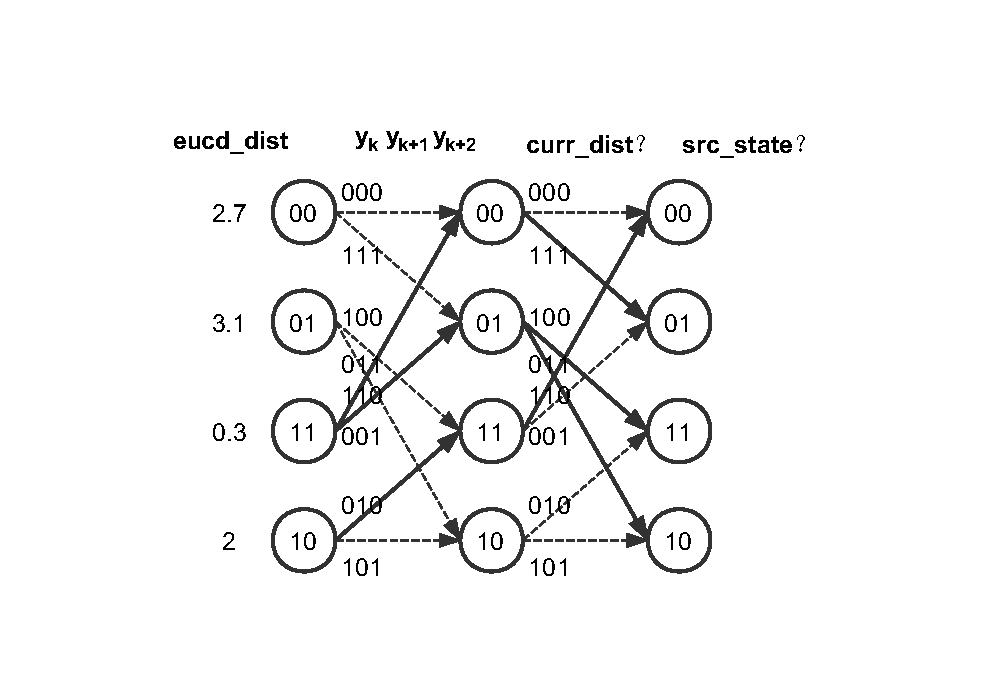
\includegraphics[width=0.6\textwidth,trim=0 40 0 40,clip]{pic/2-3-2.eps}
    \caption{(3,2)情况下软判决两步译码过程}
\end{figure}

为了解决上述的多步状态转移的情况,我们考虑将多步译码过程等效为单步译码的情况。以 (3,2)的组合为例,上图的两步译码过程可以等效地用下图中的单步译码过程表示:与两步状态转移相比,等效单步状态转移的转移路径由原来的8个变为了16个,同时,单步状态转移后所在状态可能的源状态也由原来的2个变为了4个。在实现中,我们可以使用张量积由单步转移路径矩阵生成多步转移路径矩阵,并由此计算出其相应卷积码对应的复数电平;同时,我们可以建立起一个索引数组来帮助我们快速确定多步状态转移时各路径的源状态。在完成这些操作后,我们就可以将多步状态转移过程等效地视为单步状态过程,从而用同样的思路实现其软判决译码。

\begin{figure}[h]
    \centering
    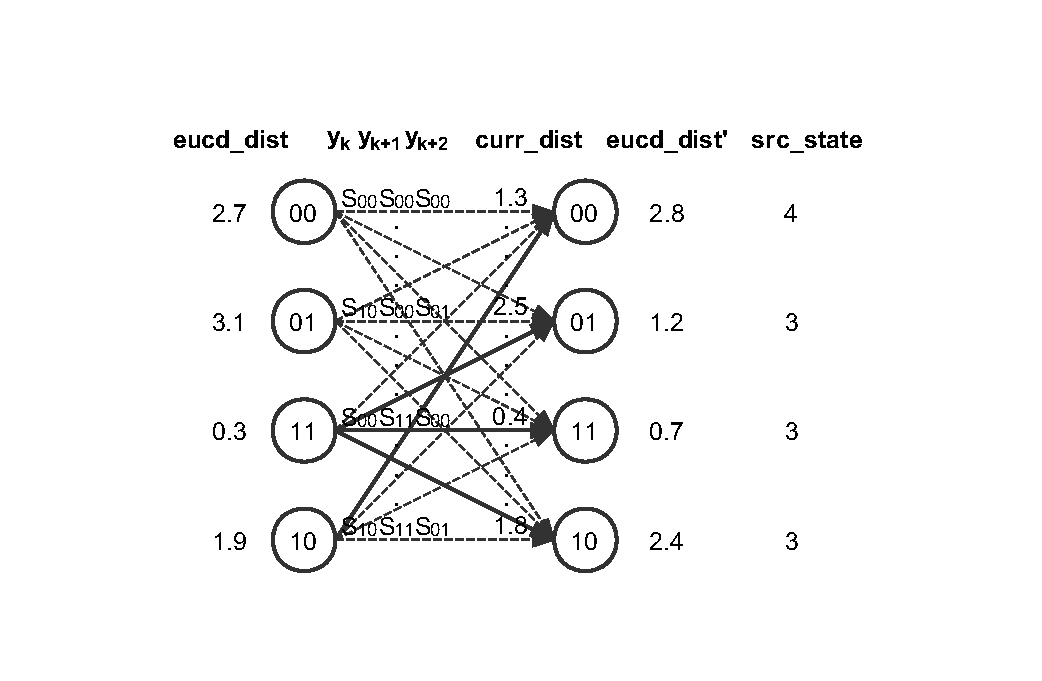
\includegraphics[width=0.6\textwidth,trim=0 40 0 40,clip]{pic/2-3-3.eps}
    \caption{(3,2)情况下软判决等效单步译码过程}
\end{figure}

\subsection{仿真分析}

在仿真中,我们生成了长度为100,000bit的随机序列,采用2bit/符号的BMPSK映射方式,设置bias\_ratio=1/4,分别作出了不进行卷积码编码,卷积码编码+硬判决译码,和卷积码编码+软判决译码的BER-SNR曲线,其中左边的图为线性坐标,右边的图为对数坐标:

\begin{figure}[h]
    \centering
    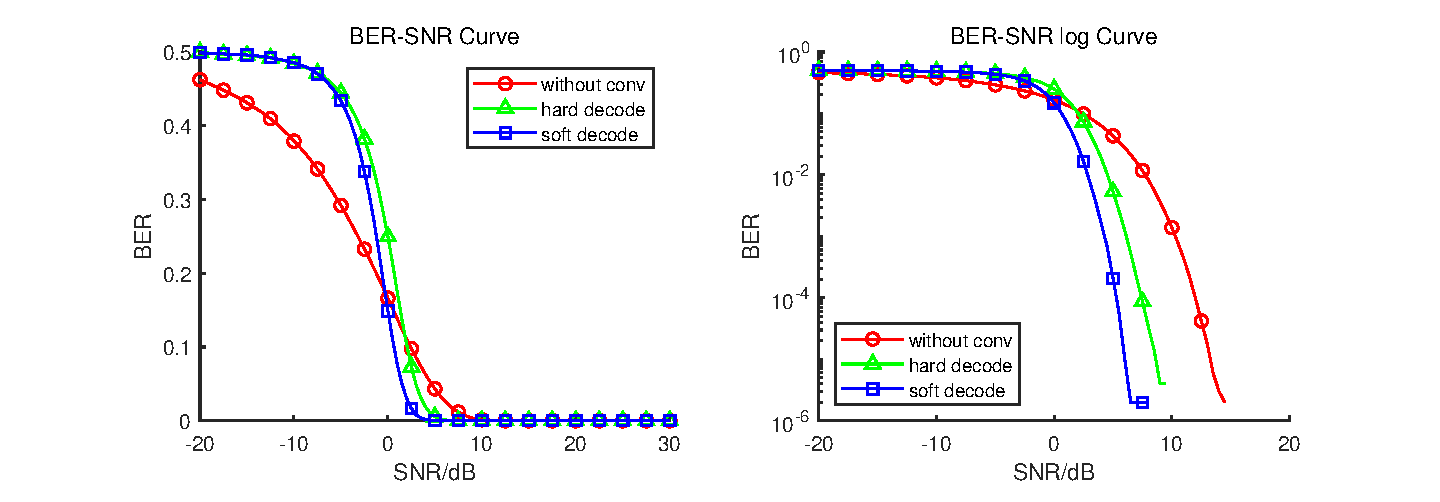
\includegraphics[width=\textwidth]{pic/2-3-4.eps}
    \caption{不卷积,硬判决,软判决时的BER-SNR曲线}
\end{figure}

对比图中代表硬判决译码的绿线和软判决译码的蓝线可以看出,在相同信噪比的条件下,软判决译码的误码率低于硬判决译码,这是因为硬判决是先将复数电平判决为比特串后,再对其进行汉明距离度量完成译码;而软判决是直接对电平进行欧氏距离度量完成译码,这种译码方式能够更加充分地利用复平面中的电平信息,因此能够获得更好的译码效果。从右边对数坐标的图中可以看出,硬判决译码的误码率在信噪比约为10dB时降至$10^{-6}$,而软判决译码的误码率在信噪比约为7dB时降至$10^{-6}$。

而观察图中代表不进行卷积码编码的红线可以发现一个有趣的现象:在信噪比较高时,经卷积编码后的误码率明显低于不进行卷积的误码率;而在信噪比较低时,卷积编码后的误码率却反而高于不进行卷积的误码率。经过分析后,我们认为出现这样的现象是由卷积码具有记忆性的特点导致的:当信噪比较高时,我们能以较高的概率译出正确的码字,由于卷积码具有记忆性的特点,因此如果出现了一个可能被误判的码字,我们仍有较大的概率通过其前后正确的码字将其正确地译码,故卷积编码后的误码率更低;而相反,在信噪比较低时,我们有较大的概率出现误判的情况,由于卷积码具有记忆性的特点,原本能正确译码的码字可能被其前后误判的码字连带地误判为错误码字,故卷积编码后误码率反而更高。

\section{CRC模块}

CRC是一个用来检错的算法,当接受到的序列$r(x)$的校正子$s(x)$非$0$,就说明序列出现了误码,但$s(x)$为$0$也不能说明一定接收到了正确的序列)。同时CRC基本没有纠错能力,但可以尝试按照一般线性码的解码纠错方法,即最小汉明判决,进行纠错。每个校正子$s(x)$都是不超过$m-1$次的多项式,因此只需要提前制作一张$2^{m-1}-1$的表,记录每个非$0$校正子对应的最轻的误码图案$e_{s(x)}(x)$,在接收后只需要对接收到的$\hat{r}(x)$进行一次求模,然后用$\hat{r}(x)$减去得到的校正子对应的最轻的误码图案即可。	
	
CRC检验的实现比较简单。输入为$k$位待编码数据和一个$m$阶生成多项式系数$g(x)$,编码结果为$n=m+k$位。其中前$k$位为信息位,直接把CRC编码模块的数据输入放在前$k$位即可。而后$m$位为校验位,结果为$d(x)x^m \mod g(x)$。这个多项式的求余可以通过MATLAB的deconv()函数实现,只需要得到正常的解卷积结果,再把余数对应的多项式投射到$2$元域上即可。生成多项式$g(x)$已经有成熟的标准,如下表所示的ITU-IEEE标准,可以直接使用。

\begin{table}[h]
    \centering
    \small
    {
        \begin{tabular}{c|c}
            \hline
                名称 & 多项式 \\
            \hline
                CRC-1 & $x+1$ \\
                CRC-3-GSM & $x^3+x+1$ \\
                CRC-4-ITU & $x^4+x+1$ \\
                CRC-5-EPC & $x^5+x^3+1$ \\
                CRC-5-ITU & $x^5+x^4+x^2+1$ \\
                CRC-5-USB & $x^5+x^2+1$ \\
                CRC-6-GSM& $x^6+x^5+x^3+x^2+x+1$ \\
                CRC-6-ITU & $x^6+x+1$ \\
                CRC-7 & $x^7+x^3+1$ \\
            \hline
        \end{tabular}
    }
    \caption{ITU-IEEE CRC生成多项式部分标准}
\end{table}

下图为0dB信噪比条件下,1/3卷积效率,1/2电平映射效率的BMPSK,CRC中一个数据块的十个典型误码图案:

\begin{figure}[h]
    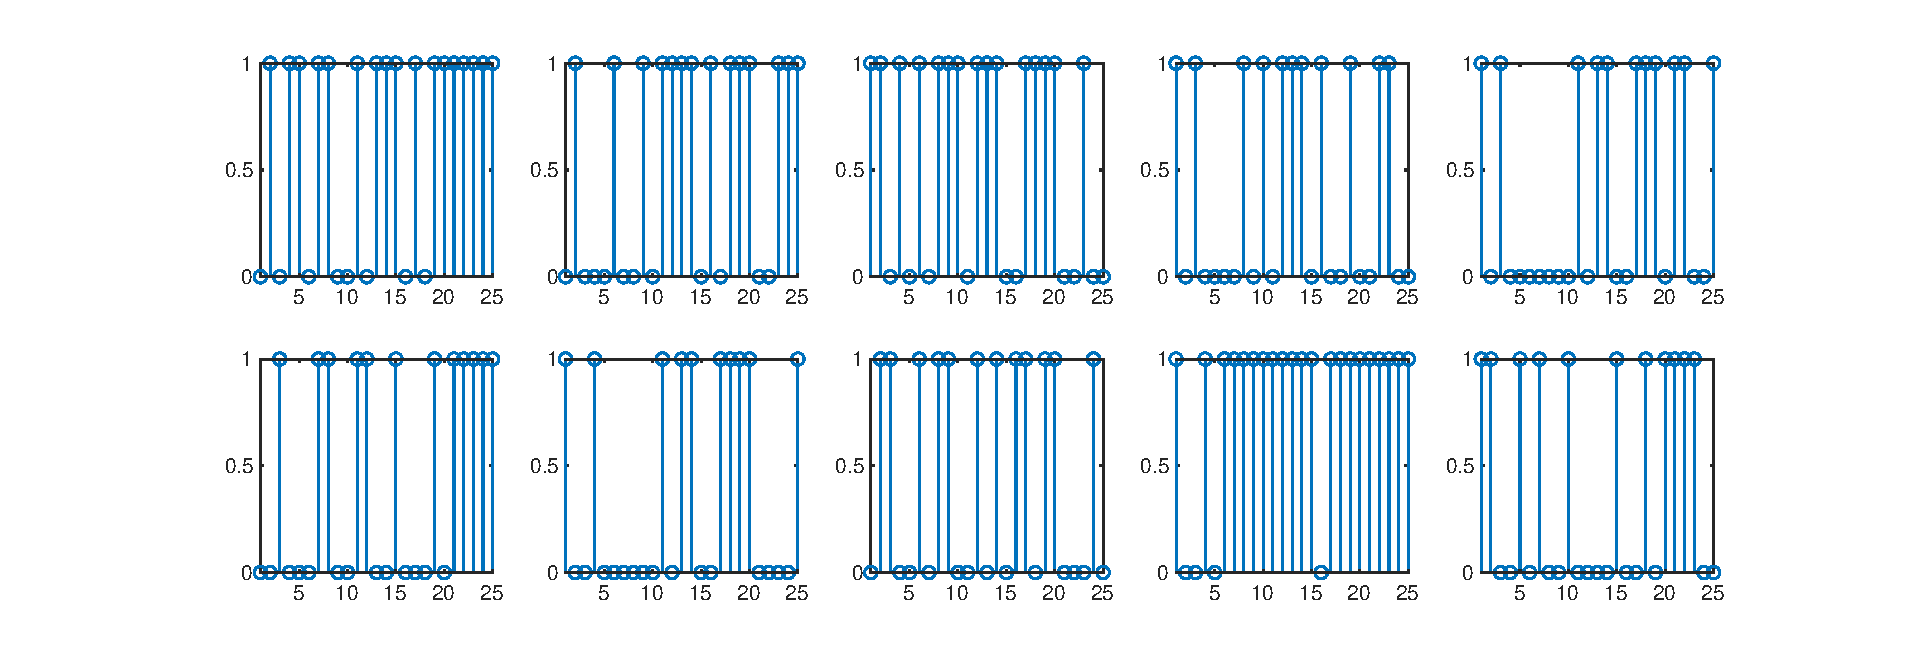
\includegraphics[width=\textwidth]{pic/pattern.eps}
    \caption{CRC误码图案}
\end{figure}

此时由于噪声较大,出现误码较多,误码图案呈随机分布。随着信噪比逐渐增加,误码率变小,误码图案也逐渐变得稀疏,直至几乎没有误码。

\section{具体任务设计}

\subsection{场景一}

场景一中,在一次通信过程,信道相位偏置$\phi$固定,传送1200bit的数据,可以使用信道的次数分别为800次、1000次、1200次、1500次、1800次,分别探究几种情况下的最佳设计。约定用以下方法对设计加以简记
\begin{center}
电平映射方法+卷积码效率+电平映射效率+训练序列长度+凿孔数目
\end{center}

其中BMPSK的训练序列长度为0,如PHIMAP+1/2+1/2+100+300表示使用PHI+MPSK电平映射,1/2效率卷积码,2bit/符号的电平映射方法, 预先发送序列100个符号,凿孔300个电平符号的设计。

在信道旋转偏置$\phi$固定的情况下,PHIMAP和BMPSK都能较好的估计出 $\phi$的值。同时,1200 bit的信息,通过1/2卷积码,会变成2400bit,再通过1电平3bit映射,会变成800个符号。这种情况下刚刚好是第一个条件下信道允许使用次数。此时要么直接使用BMPSK;要么选择通过凿孔去掉一些符号使用PHIMAP 。此时BMPSK的性能和PHIMAP性能+凿孔的效率是一样的。凿孔方法是等间隔凿孔,由于电平映射为MPSK,判决时在凿孔位置都补充为0。

使用信道次数为1000及以上时,使用信号次数比较宽裕。一般来说,卷积效率越低,卷积码的抗噪声能力越强。同时电平映射效率越低也能提高噪声能力。因此,在发送次数在1000以上的时候可以使用效率更低的卷积码和效率更低的电平映射方法。

使用信道次数为1000时。1/2效率卷积码+1/2效率电平映射,以及1/3效率卷积码+1/3效率电平映射,都需要发送1200个符号。这两种方案都相对于1/2效率卷积码搭配1/3效率电平映射有所提升。此时的BMPSK需要凿孔200个符号。同时不加卷积模块搭配1/1效率电平映射也是一种设计。因为没有卷积模块,故这1200个符号没有冗余,凿孔会给带来不可逆的损失。

使用信道次数为1200时,1/3卷积码+1/3复电平映射和1/2卷积码,以及1/3电平映射,都恰好使用信道1200次。因此BMPSK恰好使用1200次。而PHIMAP就需要凿孔来发送预先发送序列了。另外也可以采取1/1效率卷积码和1/1效率电平映射,但同样不能凿孔,因此在这种情况下只能使用BMPSK算法。

\begin{figure}[h]
    \centering
    \subfigure[800]{
        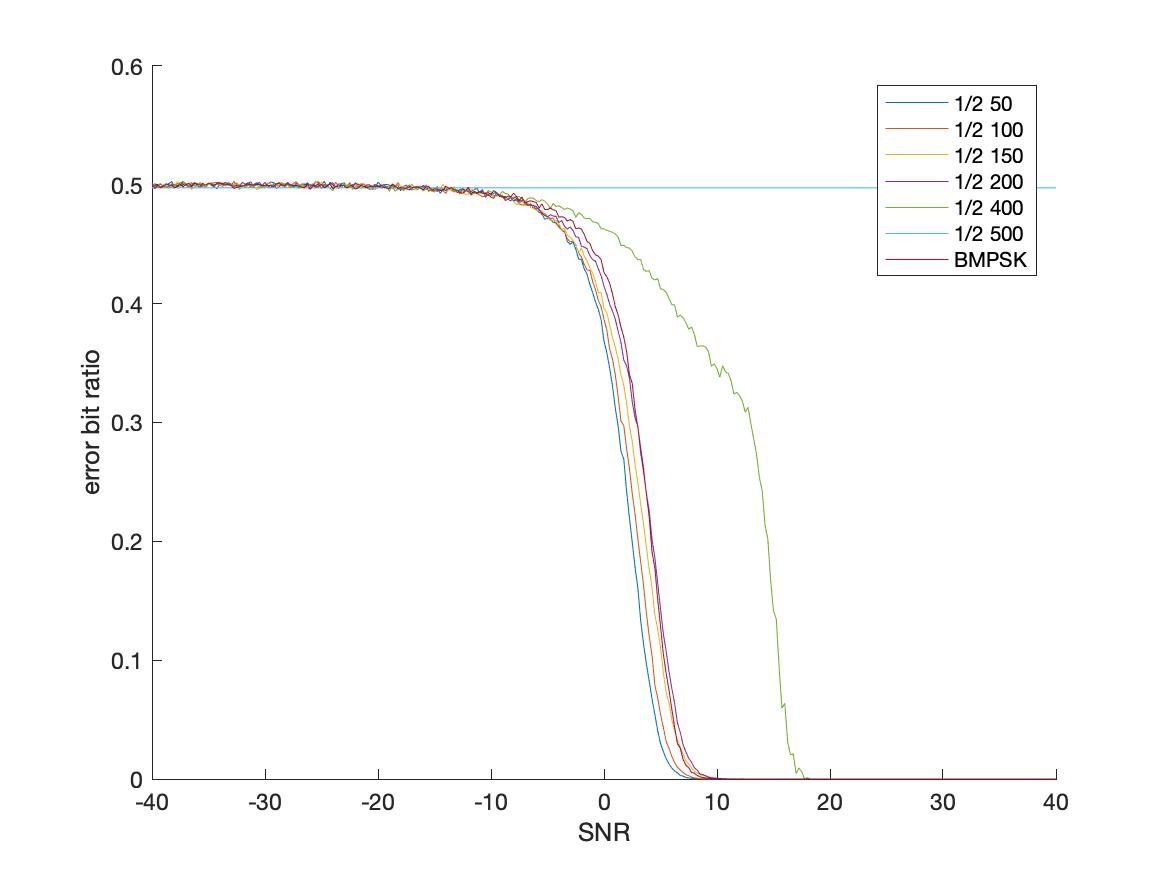
\includegraphics[width=1.9in]{pic/1_800.jpg}
    }
    \subfigure[1000]{
        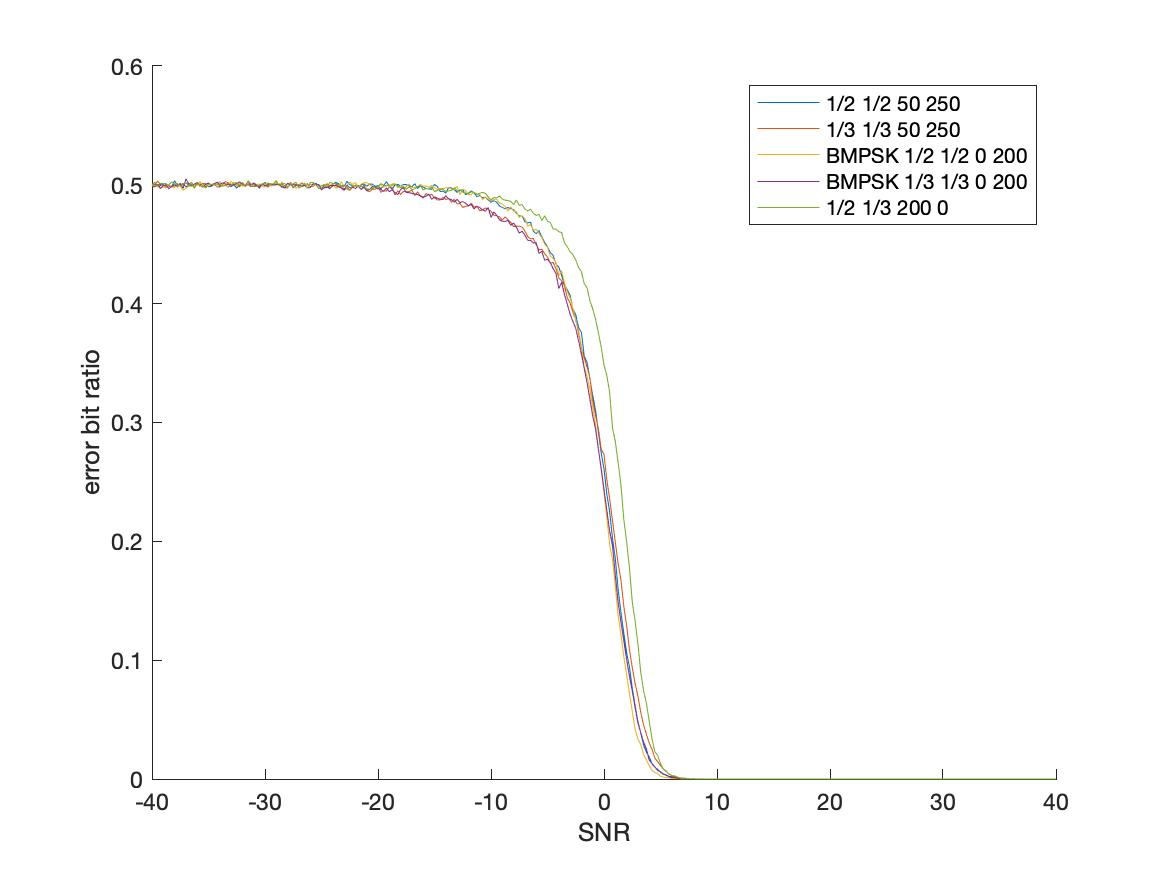
\includegraphics[width=1.9in]{pic/1_1000.jpg}
    }
    \subfigure[1200]{
        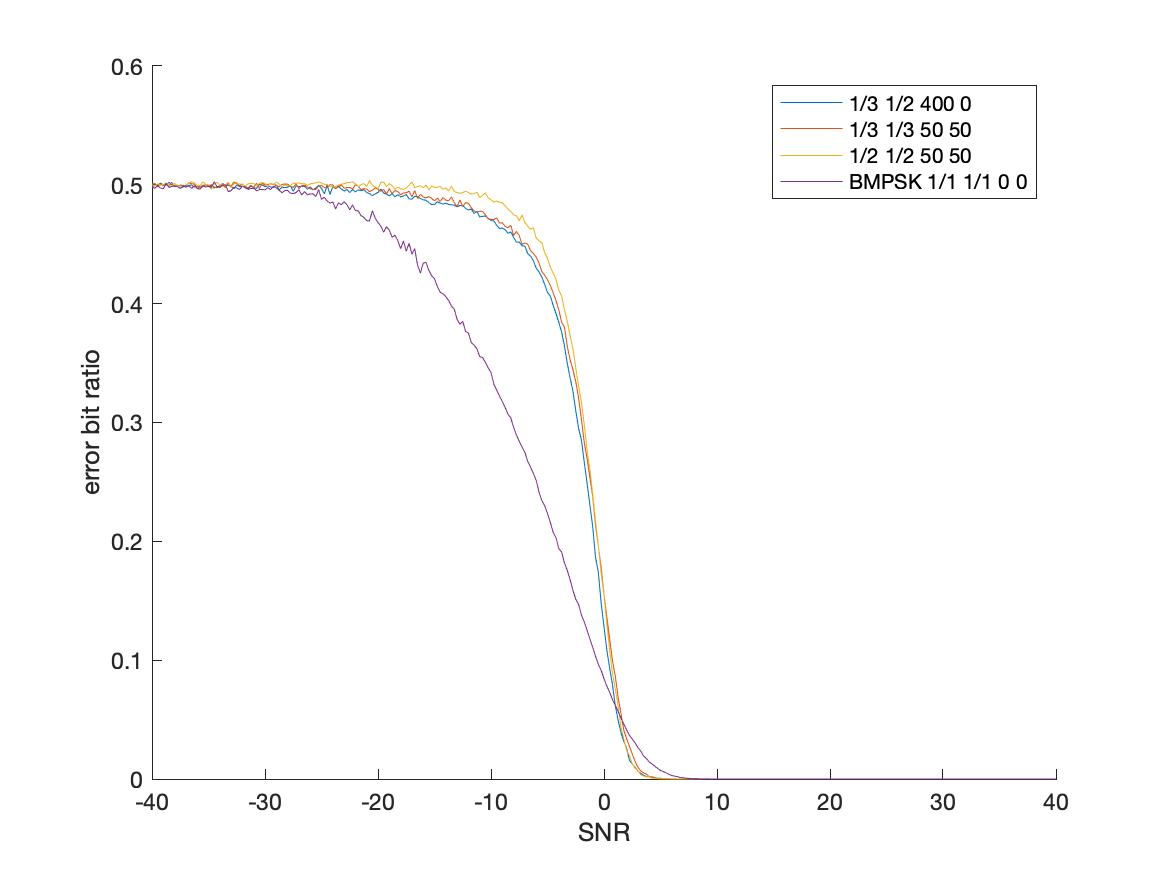
\includegraphics[width=1.9in]{pic/1_1200.jpg}
    }
    \subfigure[1500]{
        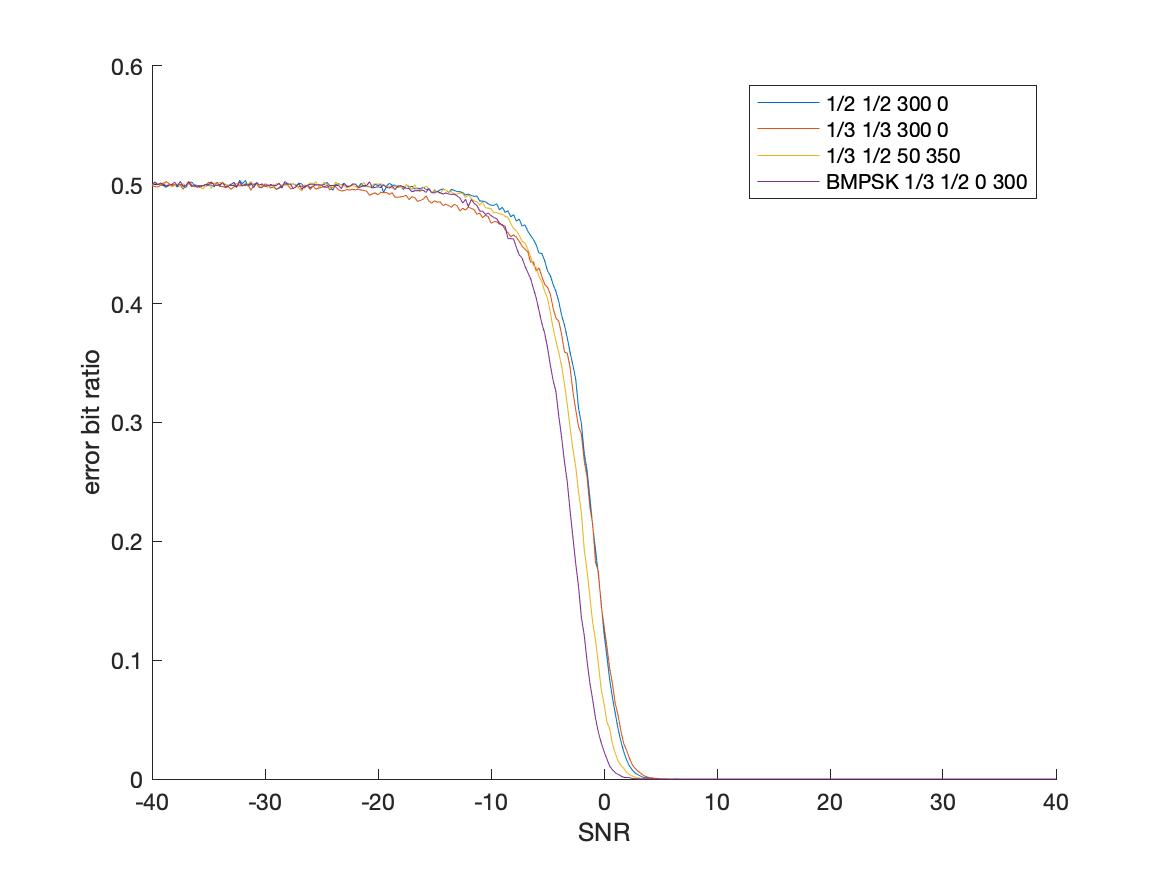
\includegraphics[width=1.9in]{pic/1_1500.jpg}
    }
    \subfigure[1800]{
        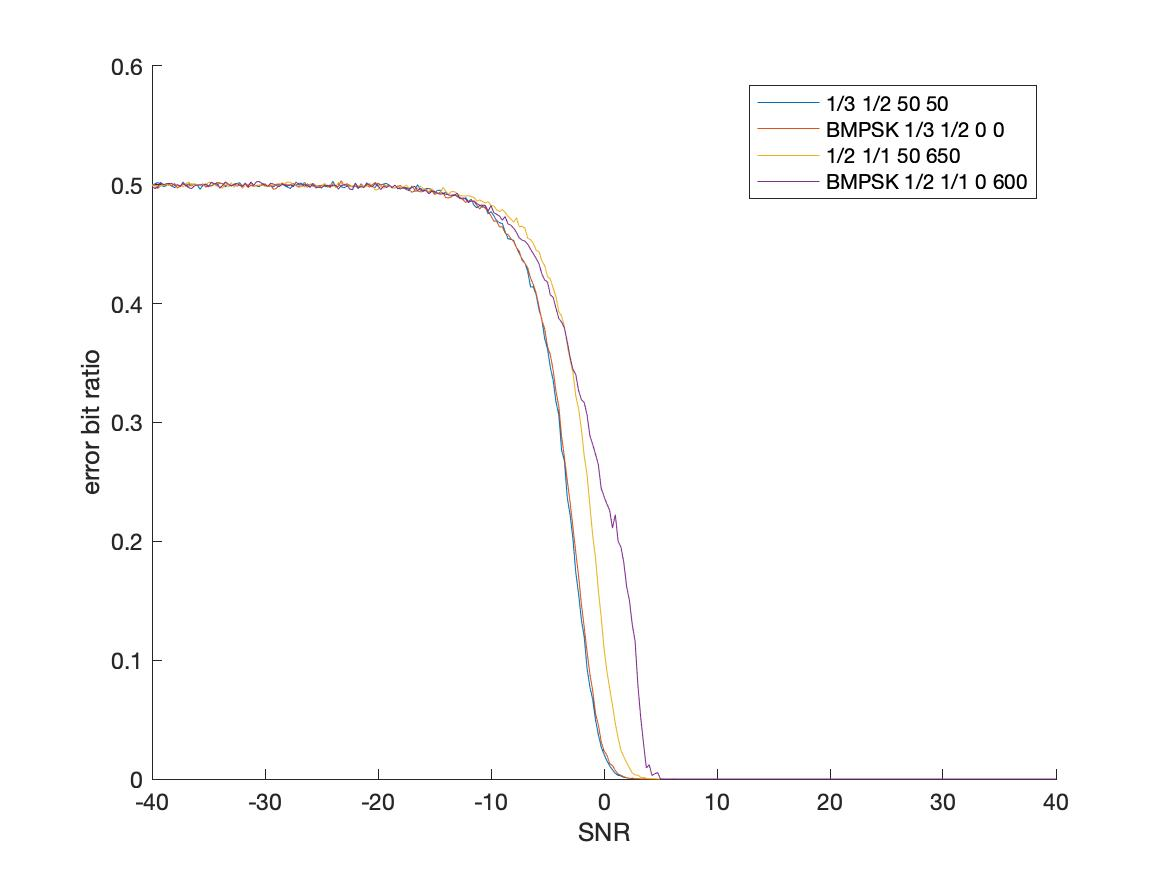
\includegraphics[width=1.9in]{pic/1_1800.jpg}
    }
    \subfigure[不同使用次数下的最佳设计]{
        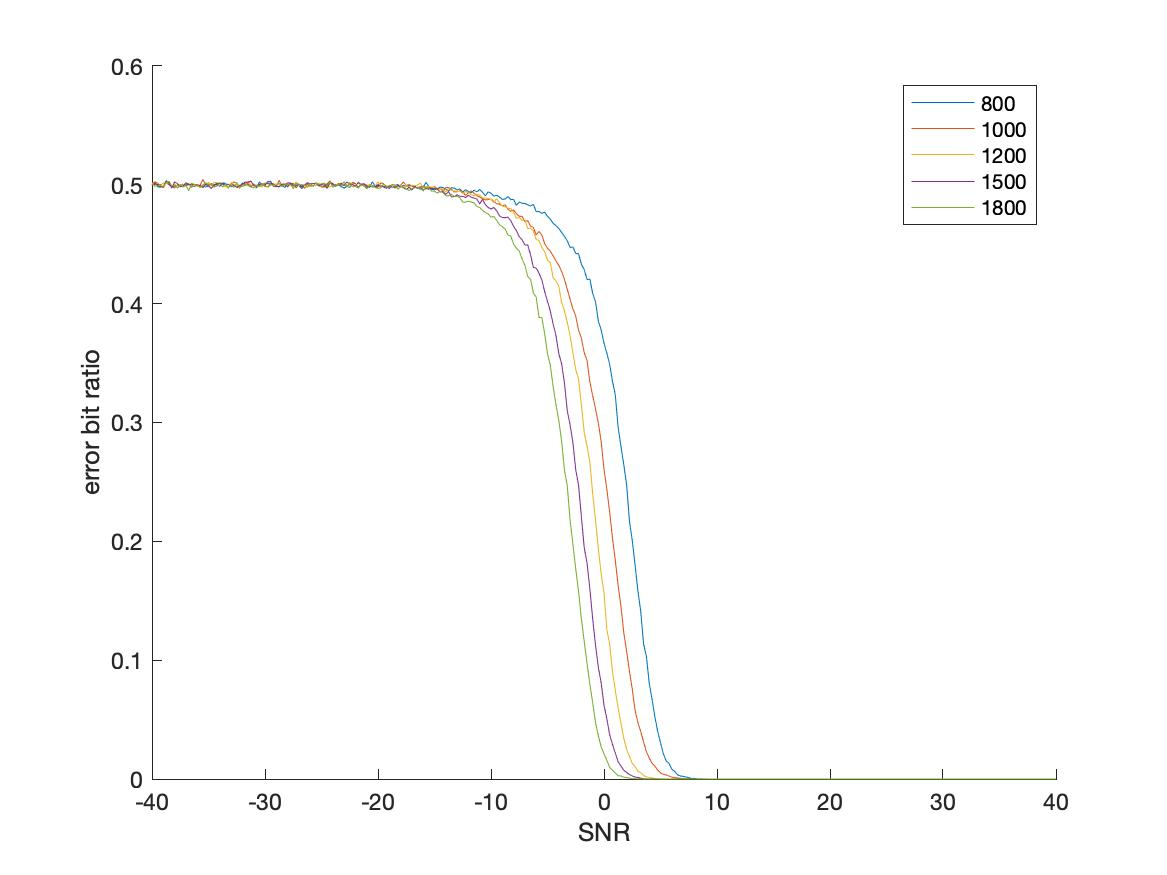
\includegraphics[width=1.9in]{pic/1_all.jpg}
    }
    \caption{场景一各种设计的SNR-BER曲线}	
\end{figure}

使用信道次数为1500时,可以使用1/3效率卷积码+1/2效率电平映射。这样我们共需要发送 1800个符号。因此,BMPSK方法和PHIMAP方法都需要凿孔。只不过需要凿300个及以上的孔,损失较大。同时可以使用1/3+1/3和1/2+1/2的方法,剩余的符号数目作为PHIMAP的训练序列,而BMPSK需要凿孔300个。

使用信道次数为1800时,使用1/3卷积码+1/2电平映射的设计就很充裕了。此时BMPSK方法无需凿孔,而PHIMAP方法也只需要凿不到100个孔,损失很小,可以对比了1/2效率卷积码+ 1/1电平映射和凿孔600的方法。

利用数值仿真可以检验各种情况下设计的合理性,同时比较出最佳设计,仿真结果如上图所示。

使用信道次数为800时,几种方法的性能相差较小。其中PHIMAP+50预发送序列+50凿孔效果最好。并且性能随着凿孔数的增加而减少。BMPSK的性能略差于凿孔数为50、100、150、200的时候。当凿孔数达到400的时候,性能恶化严重,已经在将近20dB的时候才能无损恢复。而在凿孔500个的时候,误码率一直为0.5,无法恢复。这是因为如果把1200个bit直接1/3效率电平映射得到400个电平。因此400个电平应该是能够恢复的最低电平数目。卷积码引入了冗余,因此丢失一部分电平仍然能够恢复。但是丢失了500个电平时就彻底无法恢复了。

使用信道次数为1000时,BMPSK+1/2+1/2+0+200的方法的性能最好。PHIMAP凿孔50与 BMPSK不凿孔性能一样,说明凿孔引来的性能下降是非线性的,即在相同条件下,凿孔增量带来的性能下降是随着已有凿孔数目的增长而增长的。1500的实验中也能说明这一点。除此此外,PHIMAP电平映射的方法中,降低了卷积码效率或者电平映射效率+凿孔方法的几个曲线的性能都明显优于1/2+1/3+200+0。因此说明这两个参量的对性能的影响还是很明显的。1/2+1/2的方法比1/3+1/3的方法性能略好一点,但相差很小。

使用信道次数为1200时,性能比1000个的时候有了提升。在信噪比小于SNR<0.25dB的时候,BMPSK+1/1+1/1+0+0的方案明显优于其他方案。因此如果信道环境非常恶劣,低于0dB的时候,最后一种方案的结果将明显好于其他方案。

使用信道次数为1500时,性能比1200个的时候有了提升。同时仿真结果也再次说明了凿孔引来的性能下降是非线性的,即在相同条件下,凿孔增量带来的性能下降是随着已有凿孔数目的增长而增长的。

使用信道次数为1800时,性能比1500个的时候有了较为明显的提升。可以说明凿孔数量太多对性能有着较大的影响。1/2+1/1的搭配的性能并不好也可以印证这一点。

整理得到各种情况下的最优设计如下:

\begin{table}[h]
    \centering
    \small
    \begin{tabular}	{|c|c|}
        \hline
            使用信道次数&最优设计 \\ 
        \hline
            800& PHIMAP+1/2+1/3+50+50 或 BMPSK+1/2+1/3+0+0\\
            1000& BMPSK+1/2+1/2+0+200 或 BMPSK+1/2+1/2+50+250\\
            1200& PHIMAP+1/2+1/2+50+50 或 BMPSK+1/2+1/2+50+50\\
            1500& BMPSK+1/3+1/2+0+300 或 BMPSK+1/3+1/2+50+350\\
            1800& PHIMAP+1/3+1/2+50+50 或 BMPSK+1/3+1/2+0+0\\
        \hline
    \end{tabular}
    \caption{场景一下的最优设计}
\end{table}

总的来看,在其他条件相同的情况下,凿孔数目越多,性能下降越大。并且,凿孔引来的性能下降非线性的,即在相同条件下,凿孔增量带来的性能下降是随着已有凿孔数目的增长而增长的。凿孔数目超过待传输比特数和电平映射效率的乘积时,几乎无法恢复出任何信息,误码率为0.5。PHIMAP在训练序列达到50个的时候,就已经不会带来什么误差了。在给定信噪比、卷积效率、电平映射效率以及不允许多发送符号数的情况下,BMPSK的性能和少量凿孔(50)的PHIMAP的性能一样。但凿孔过多的时候,BMPSK的性能会更好一些。

\subsection{场景二}

场景二中,在一次通信过程,信道相位偏置$\phi$随机变化,传送1200bit的数据,可以使用信道的次数分别为800次、1000次、1200次、1500次、1800次,分别探究几种情况下的最佳设计。此时映射方式只能使用ASK,约定用以下方法对设计加以简记:
\begin{center}
卷积码效率+电平映射效率+凿孔数目
\end{center}

其中BMPSK的训练序列长度为0,如1/2+1/2+100表示使用PHI+MPSK电平映射,1/2效率卷积码,2bit/符号的电平映射方法,凿孔100个电平符号的设计。

使用信道次数为1000及以下时,大体只有两种设计方法。一种是1/2+1/3+0,使得使用信道次数限制在800次,另一种则是使用相匹配的编码效率和映射效率,得到1200个符号,再通过凿孔进行压缩。凿孔的位置在判决时都补充为$\frac{A}{2}$,即电平符号的期望。

使用信道次数为1200时,没有必要进行凿孔,只需要使用相匹配的编码效率和映射效率,得到1200个符号。1/1+1/1+0,1/2+1/2+0和1/1+1/1+0都是可能的设计。

使用信道次数为1500时,1/3+1/2+300是一种可行的设计。这样我们一共需要发送1800个符号,还需要凿300个孔。也可以使用相匹配的编码效率和映射效率,得到1200个符号。但这样会浪费300次使用信道的机会。或者只用1200次信道,和前一种一样。
    
使用信道次数为1800时,1/3+1/2+0和1/2+1/1+600都是可行的设计,需注意的是后者虽然因编码效率较低带来了大量冗余,但凿孔数目过多,占到了四分之一,故性能可能会比较一般。

\begin{figure}[h]
    \centering
    \subfigure[800]{
        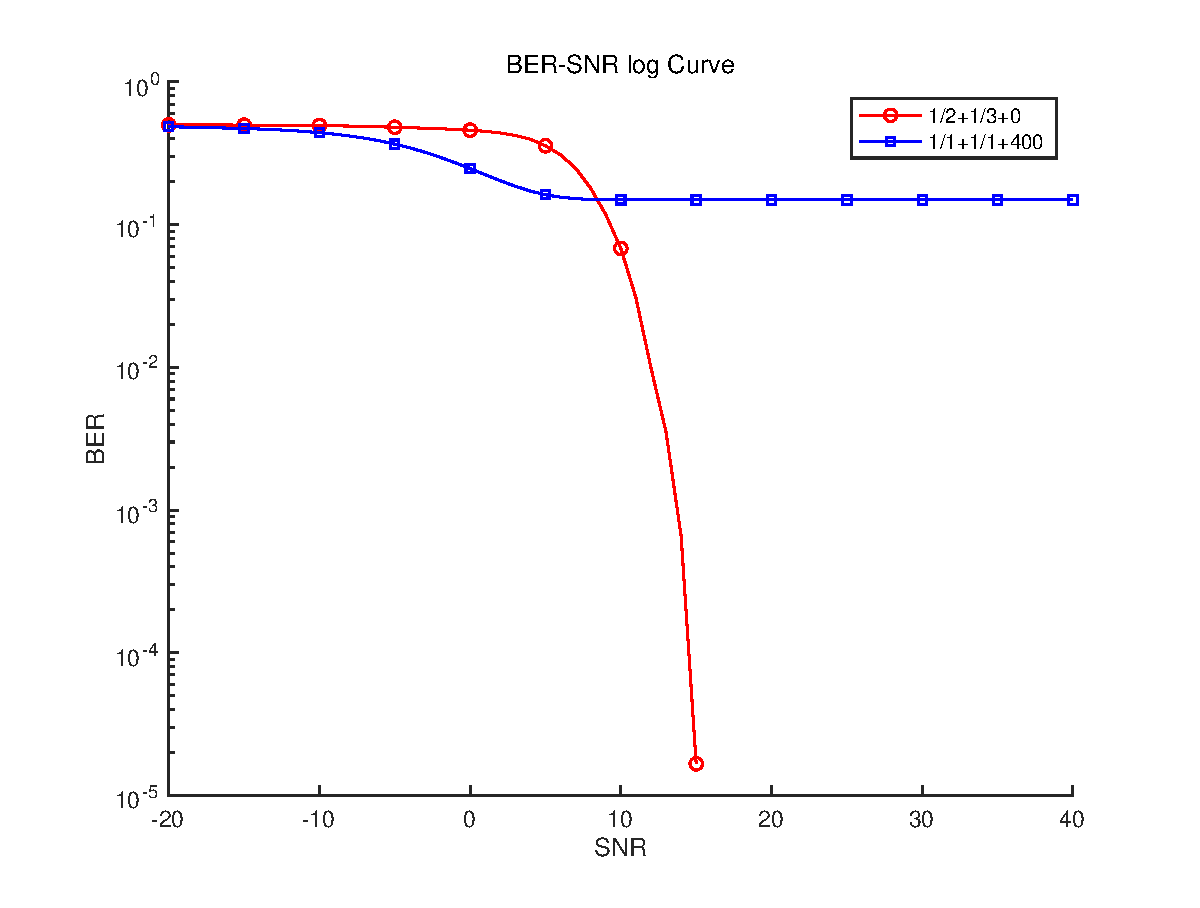
\includegraphics[width=1.8in]{pic/2_800.eps}
    }
    \subfigure[1000]{
        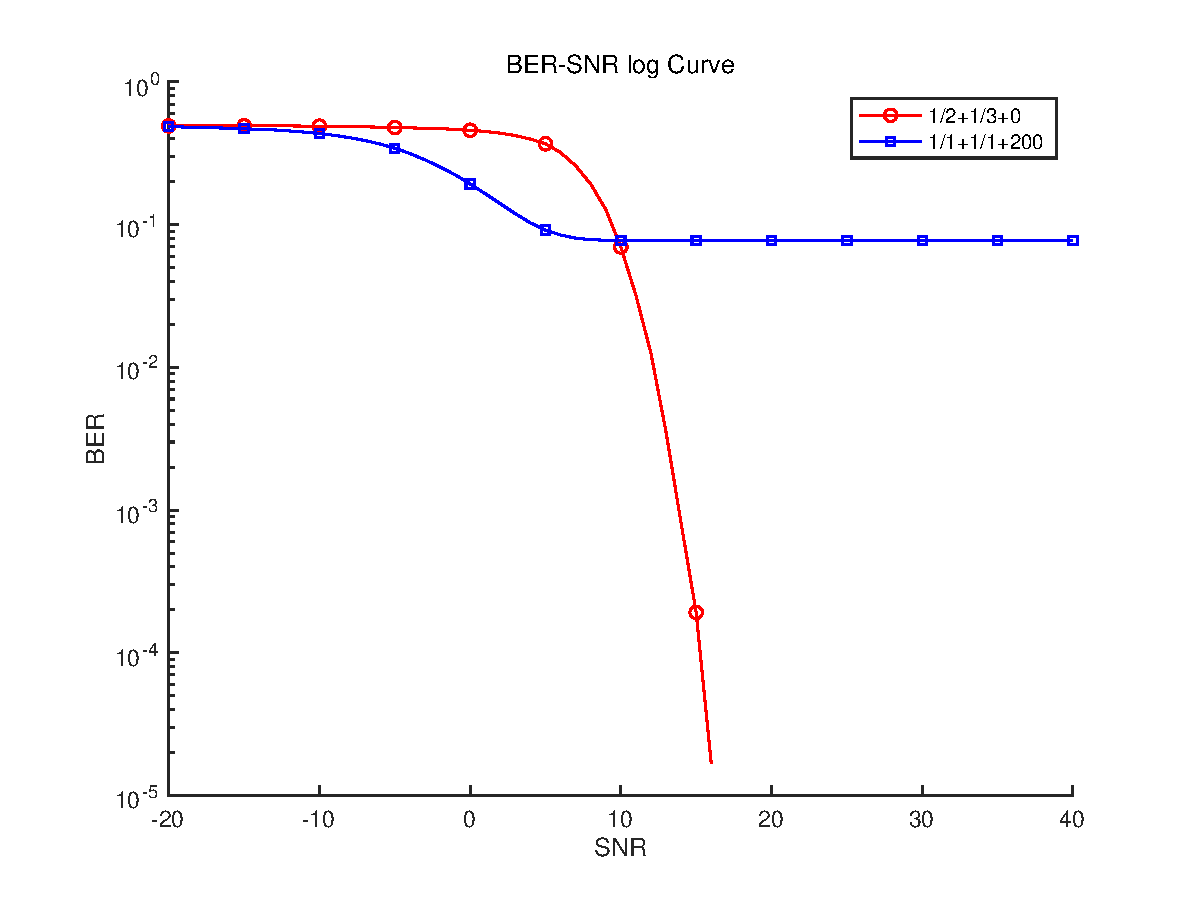
\includegraphics[width=1.8in]{pic/2_1000.eps}
    }
    \subfigure[1200]{
        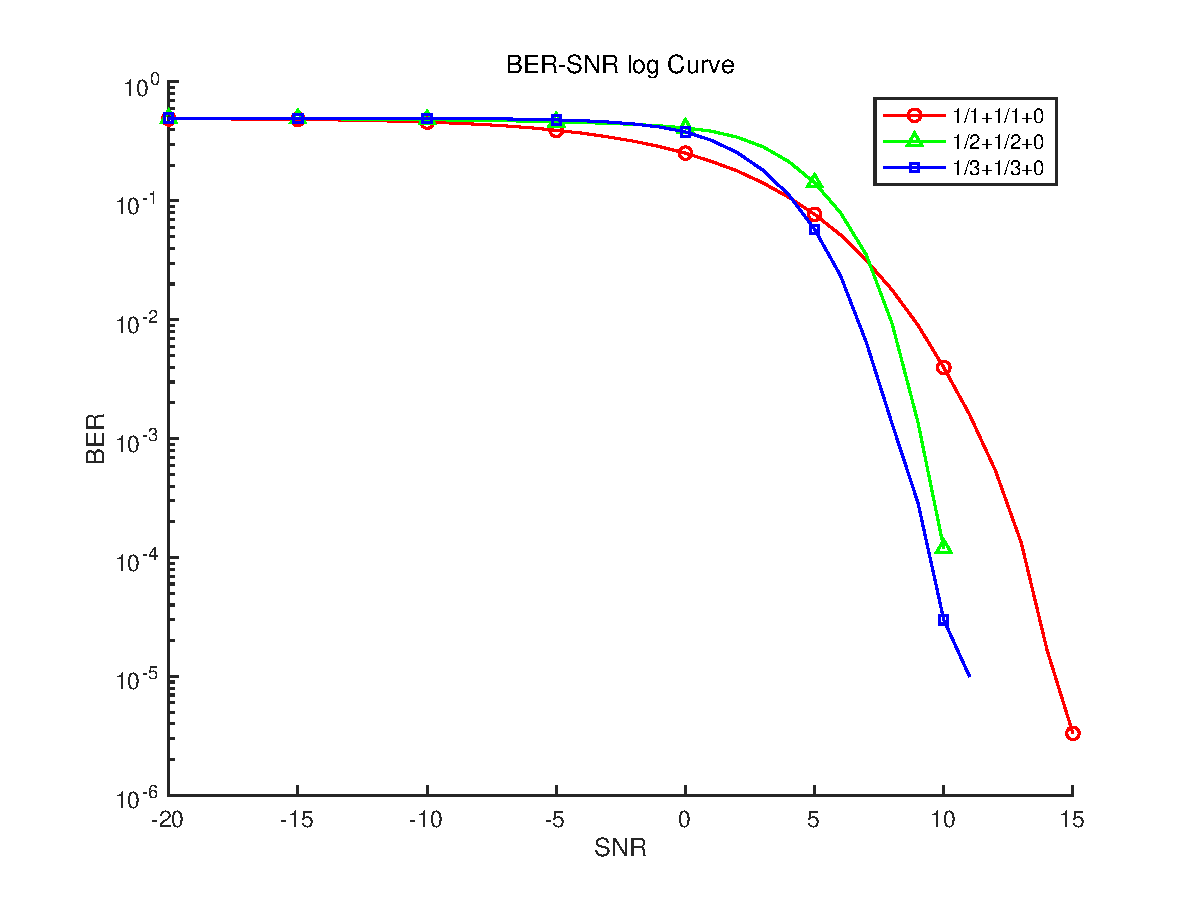
\includegraphics[width=1.8in]{pic/2_1200.eps}
    }
    \subfigure[1500]{
        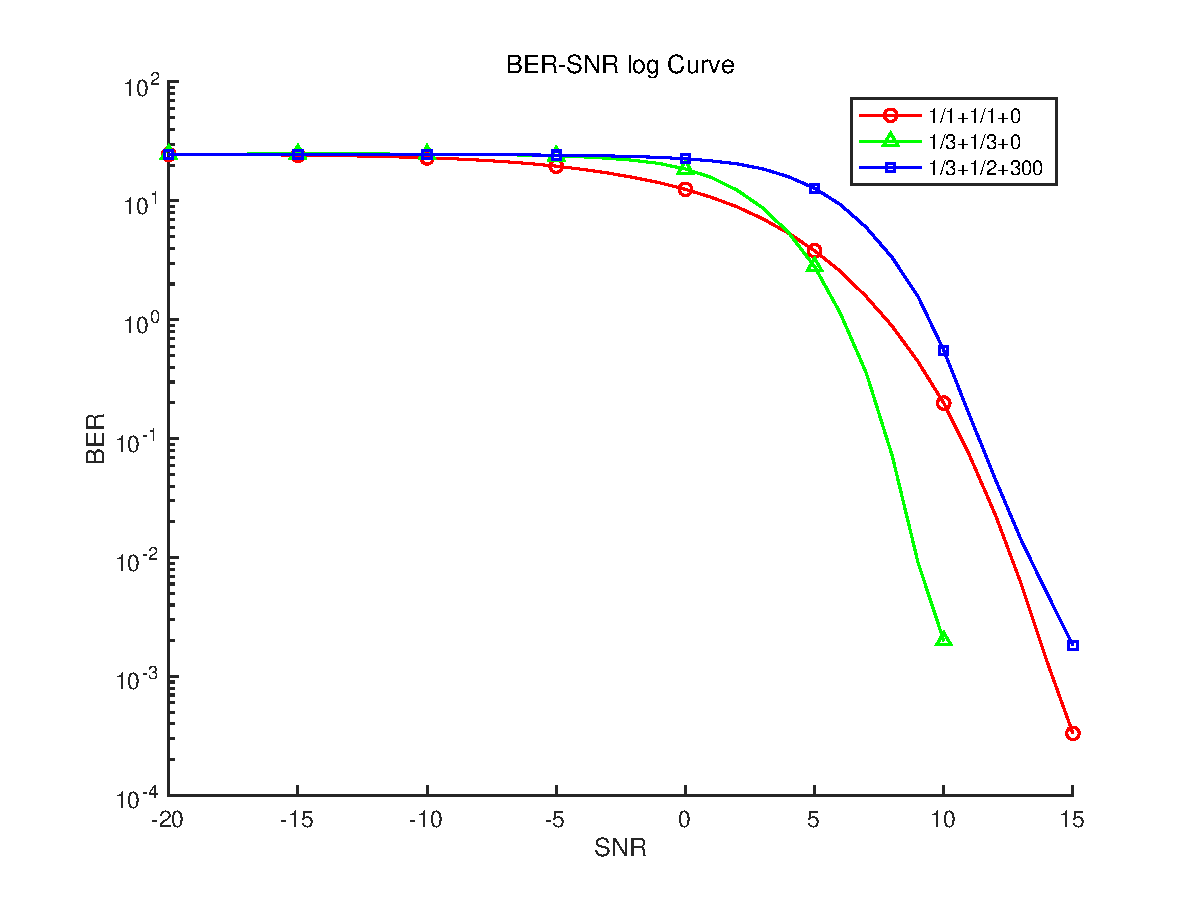
\includegraphics[width=1.8in]{pic/2_1500.eps}
    }
    \subfigure[1800]{
        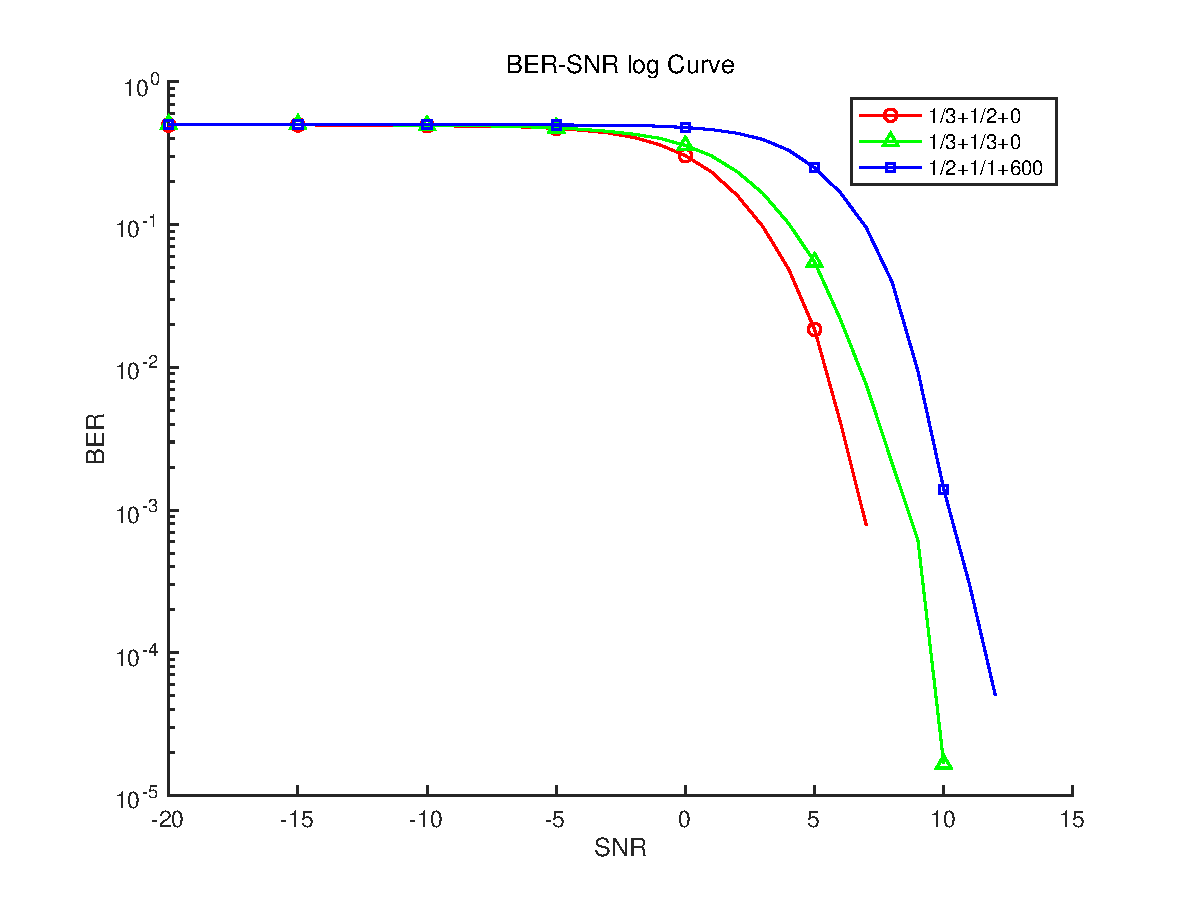
\includegraphics[width=1.8in]{pic/2_1800.eps}
    }
    \subfigure[不同使用次数下的最佳设计]{
        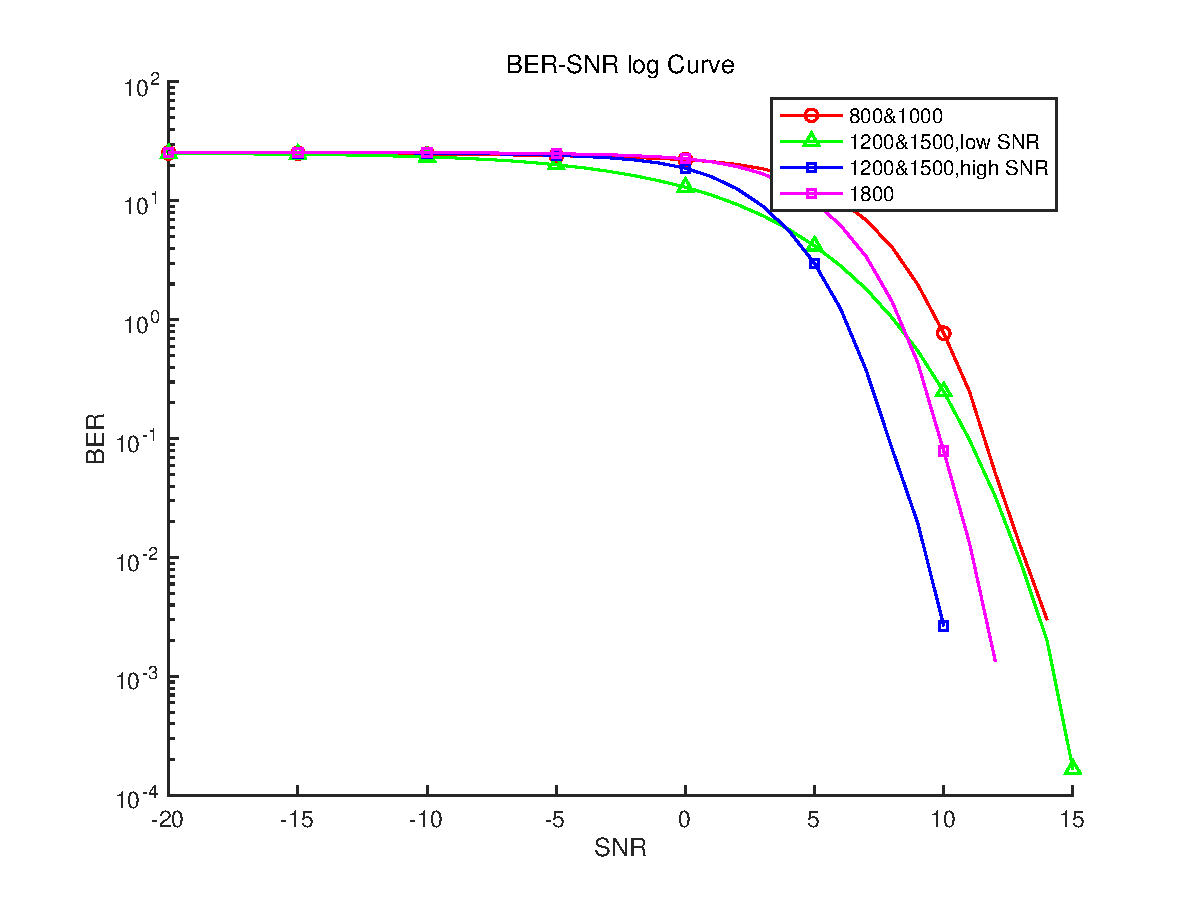
\includegraphics[width=1.8in]{pic/2_all.eps}
    }
    \caption{场景二各种设计的SNR-BER曲线}	
\end{figure}

利用数值仿真可以检验各种情况下设计的合理性,同时比较出最佳设计,仿真结果如上图所示。

使用信道次数为800或1000时,可以发现凿孔会使得误码率分别收敛于0.1492和0.0775,此时凿孔数目分别为400和200,占到了总电平符号数的三分之一和六分之一,可以视为凿掉的部分的误码率为0.5,完全无法恢复。因此可能导致误码率无法下降,在这种情况下,1/2+1/3+0的设计只需要使用800次信道,是唯一可能的选择。
    
使用信道次数为1200时,没有必要进行凿孔,只需要使用相匹配的编码效率和映射效率,得到1200个符号。1/1+1/1+0,1/2+1/2+0和1/3+1/3+0都是可能的设计。三者相比,1/1+1/1+0 在低信噪比时表现更好,而1/3+1/3+0在高信噪比时表现更好,这与之前对卷积码分析得到的结论一致,低效率的卷积增加了比特的信息冗余,信噪比较高时判决和解码的可以有更多可靠的信息参考,信噪比较低时则会参考更多错误的信息,导致错误蔓延。

使用信道次数为1500时,1/3+1/2+300的性能甚至要比只用1200次信道的1/3+1/3+0 还要差,300的凿孔数目占到了总电平符号数的五分之一是导致性能下降的原因之一。这种情况下最好的设计就是浪费300次的使用信道次数,根据信噪比的大小选择1/1+1/1+0或1/3+1/3+0。
    
使用信道次数为1800时,1/2+1/1+600的凿孔数目占到了四分之一,从之前几组的情况来看性能不会很好,仿真的结果也可以印证这一点,因此恰好使用信道1800次且不凿孔的1/3+1/2+0 即为最优设计。

相对于场景一,场景二可以利用剩余使用信道次数的方法不多,映射的选择也非常单一,而且仿真的结果表明凿孔也不适用于ASK。当凿孔数目占到总资源数的约五分之一时,性能就会明显地下降。另一个发现是,如果凿孔后的信道数用次数小于待发送的的比特数,则误码率随着信噪比增高会收敛在个凿孔数目在总电平符号数目占比的一半附近,即凿掉部分的误码率为0.5,凿孔带来了无法恢复的影响。造成这种情况的一个可能原因是判决时所有的凿孔位置都补充为$\frac{A}{2}$,在非1bit/符号的情况下无法保证到各电平的距离相等,因此会更倾向于判决成靠近$\frac{A}{2}$的值。但是仿真中可以观察到在1bit/符号的情况下凿孔的性能同样不够好,说明之前在判决时的偏差可能只是次要因素。

总而言之,根据信噪比情况选择合适的编码效率与电平映射效率就能得到相对最优的设计。在实际情况下,还可以利用CRC进行检错,收端将发生错误的块回传给发端,要求发端重传,这也是利用富裕的信道资源降低误码率的方法,由于篇幅有限,这里暂不给出仿真结果和理论分析。

整理得到各种情况下的最优设计如下:
\begin{table}[h]
    \centering
    \small
    \begin{tabular}	{|c|c|}
        \hline
            使用信道次数&最优设计 \\ 
        \hline
            800& 1/2+1/3+0\\
            1000& 1/2+1/3+0\\
            1200& 1/1+1/1+0\ 或 1/3+1/3+0\\
            1500& 1/1+1/1+0\ 或 1/3+1/3+0\\
            1800& 1/3+1/2+0\\
        \hline
    \end{tabular}
    \caption{场景二下的最优设计}
\end{table}
